%% The following is a directive for TeXShop to indicate the main file
%%!TEX root = diss.tex

\chapter{Interpretation of 3D Reconstruction Model}
\label{ch:3DRecon_Interp}
In order to validate the 3D reconstruction taxonomy and the model derived from it, interpretability from the object centric model into appropriate solutions must be shown. Our interpreter is based on the direct evaluation of the performance of each 3D reconstruction algorithm under different conditions presented in Chapter~\ref{ch:3DRecon_Benchmark}. From this analysis of how algorithms perform on objects which have different visual and geometric properties, an algorithm(s) can be definitively chosen based on which performed best on the training images.

The three algorithms introduced in our test bench are: the PMVS proposed by \citeauthor{furukawa2010accurate}, the example-based Photometric Stereo proposed by \citeauthor{hertzmann2005example}, and a standard gray-coded Structured Light technique with error rejection.

Although there are only three algorithms selected, all of them are the top performers in the corresponding field, and are sufficient to demonstrate the framework's ability to translate the descriptive model into a reconstruction. The integration of a new algorithm requires only that they be evaluated with a similar procedure and images presented in Chapter~\ref{ch:3DRecon_Benchmark}, allowing researchers to contribute novel algorithms to the framework. The source code and blender files used to generate the images are available online to encourage the testing of additional algorithm, and incorporation of additional properties.

\section{Synthetic Datasets}
We use three objects shown in Figure~\ref{fig:synth_data}, and four property lists in Table~\ref{tab:prop_list_synth_data} to test the validity of the abstraction. All four cases are labeled in Figure~\ref{fig:training_labeled} so that it would be easier to check which technique(s) give a good reconstruction based on our abstraction.

\begin{table}[h]
  \centering
  \begin{tabular}{l*{5}{c}}
  \hline
  \textbf{Property} & Texture & Albedo & S/D ratio & Roughness & Best-suited techniques\\
  \hline
  (a) & 0.2 & 0.2 & 0.2 & 0.5 & MVS, SL\\
  (b) & 0.2 & 0.8 & 0.2 & 0.5 & MVS, SL, PS\\
  (c) & 0.8 & 0.2 & 0.2 & 0.5 & MVS\\
  (d) & 0.2 & 0.2 & 0.8 & 0.2 & PS\\
  \hline
  \end{tabular}
  \label{tab:prop_list_synth_data}
  \caption{Property lists of the test objects. Link to the labels in Figure~\ref{fig:training_labeled}, (a): dark blue rectangle, (b): dark green rectangle, (c): light blud rectangle, (d): light green rectangle.}
\end{table}

\begin{figure}[h!]
\centering
\begin{tabular}{ccc}
  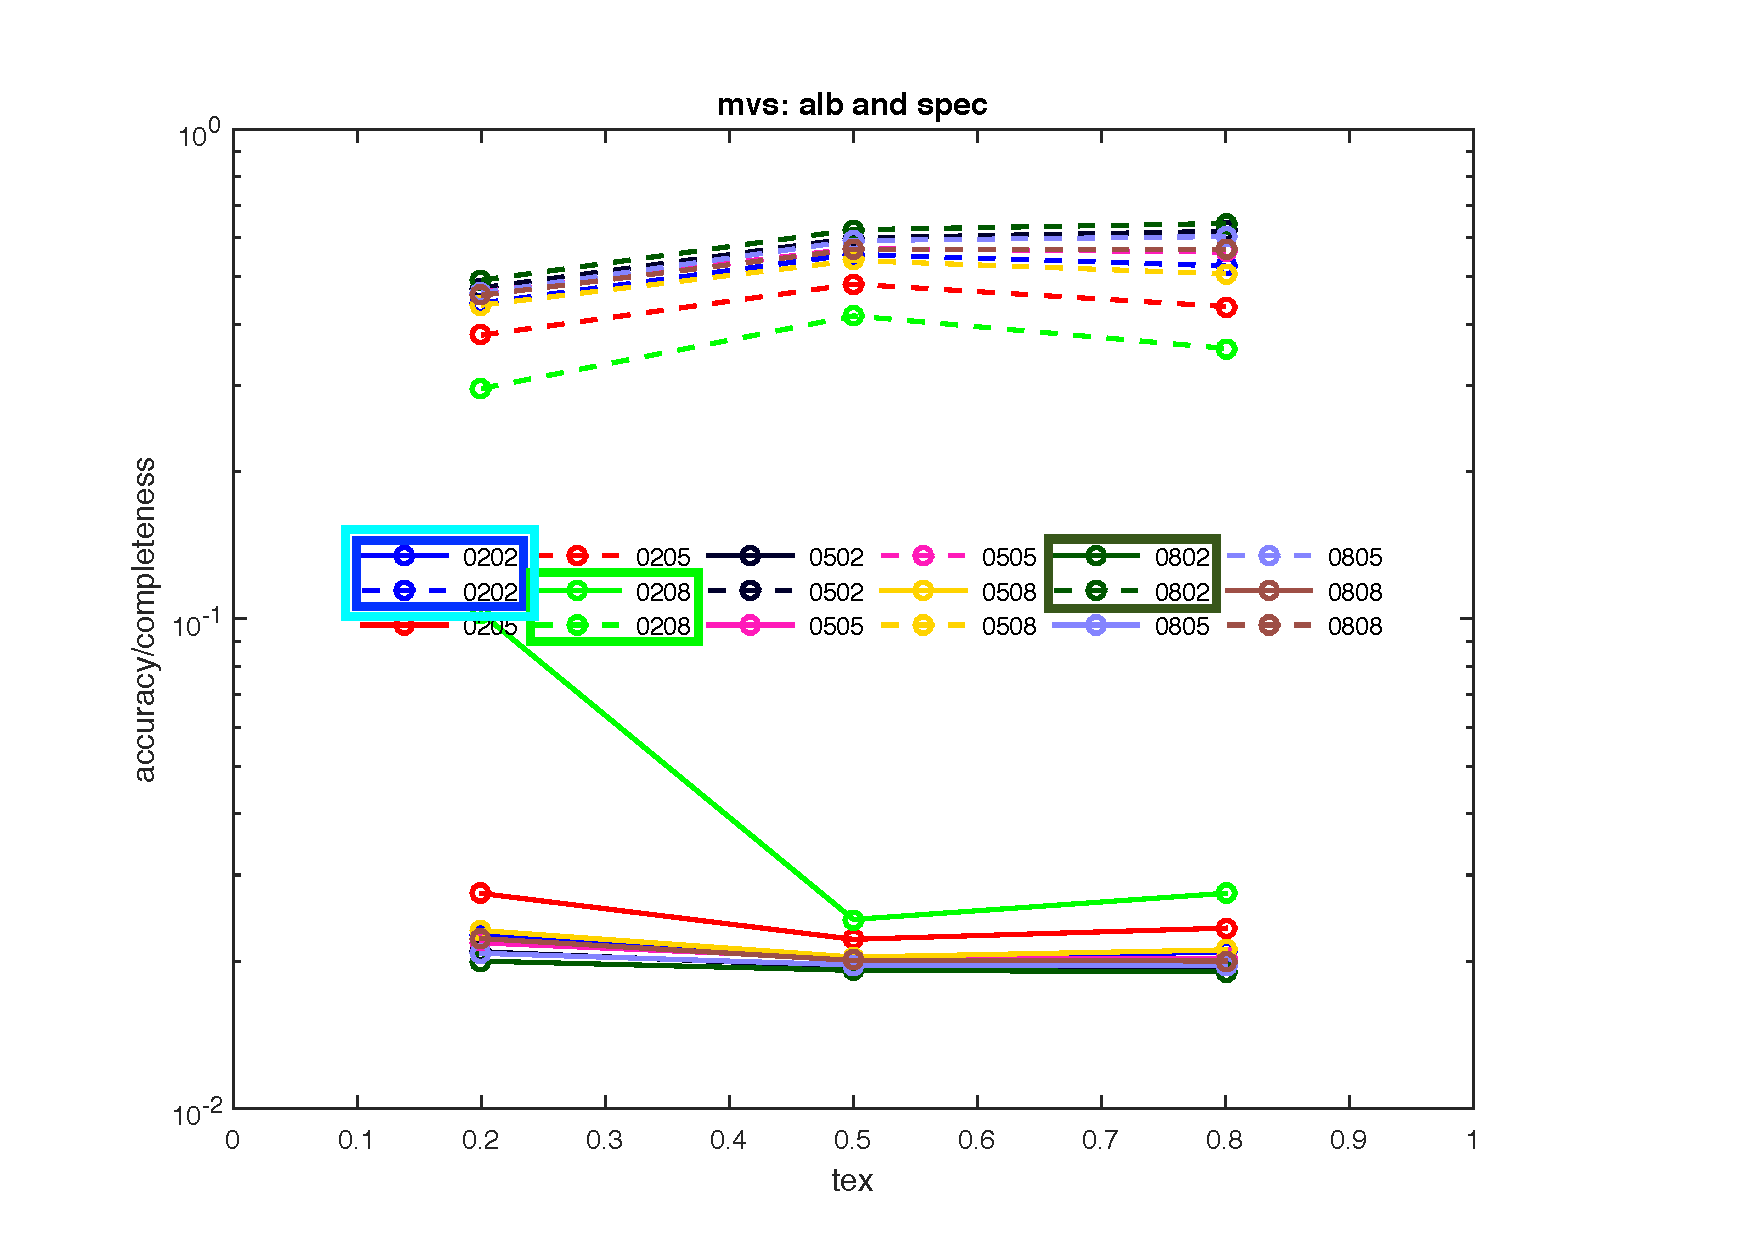
\includegraphics[width=0.33\textwidth]{interp/synth_data/mvs_train_label}&
  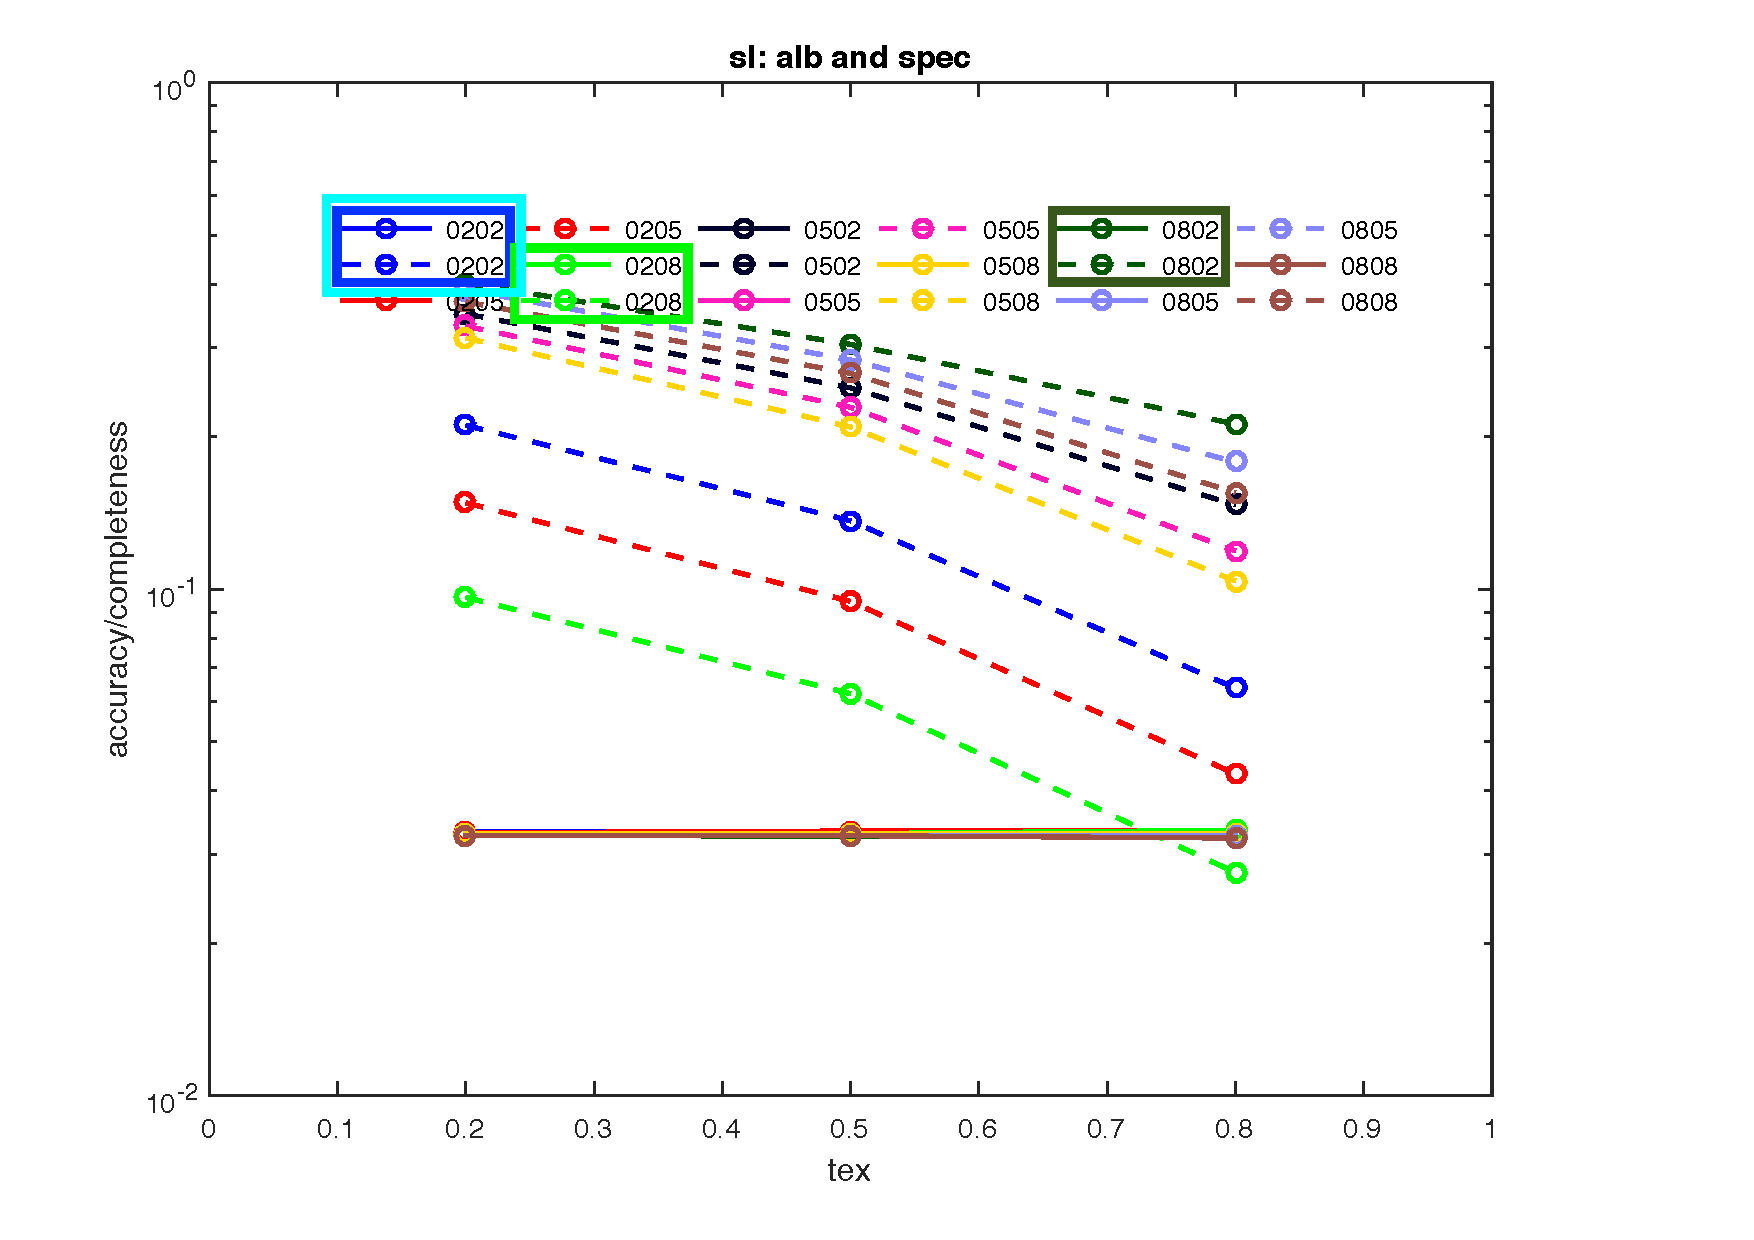
\includegraphics[width=0.33\textwidth]{interp/synth_data/sl_train_label}&
  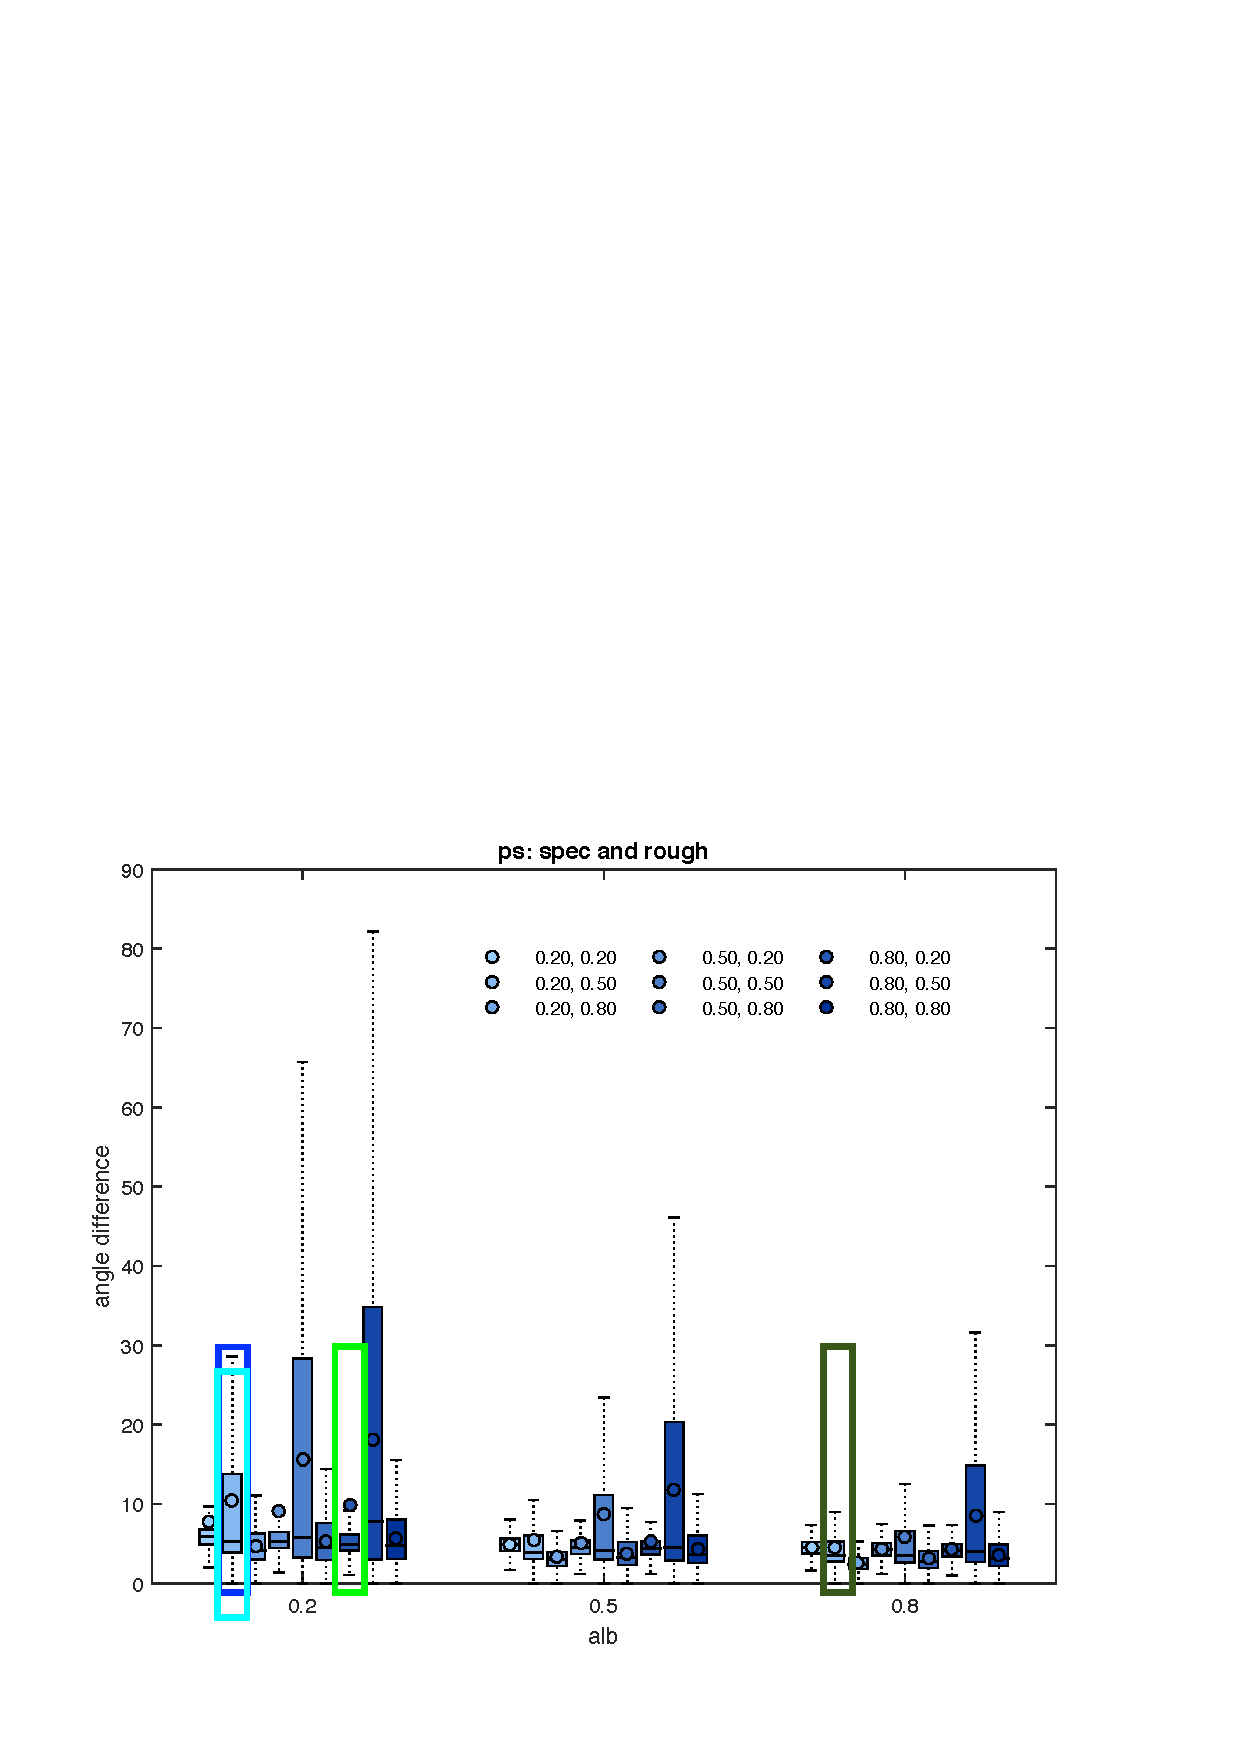
\includegraphics[width=0.33\textwidth]{interp/synth_data/ps_train_label}\\
\end{tabular}
\caption{Performance of MVS, Sl and PS with varied properties.}
\label{fig:training_labeled}
\end{figure}

\begin{figure}[h!]
\centering
\begin{tabular}{ccc}
  Cup & Pot & Vase\\
  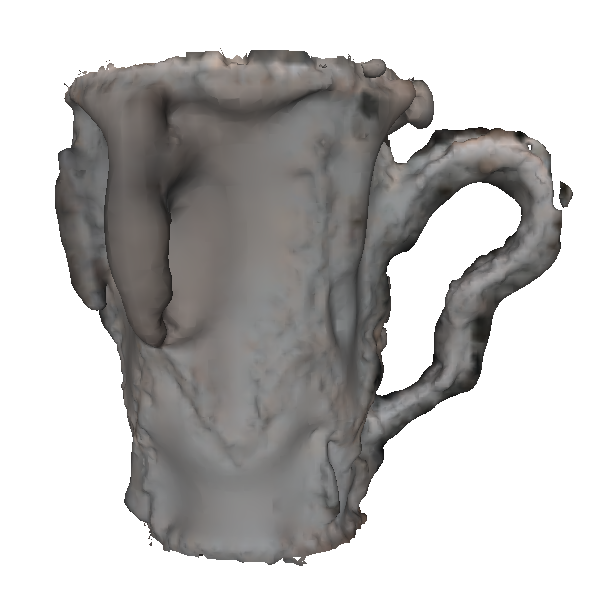
\includegraphics[width=0.33\textwidth]{interp/synth_data/cup/cup_mvs}&
  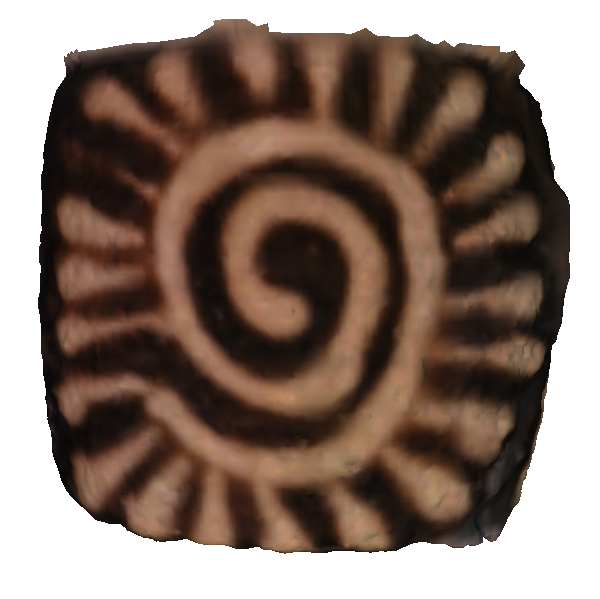
\includegraphics[width=0.33\textwidth]{interp/synth_data/pot/pot_mvs}&
  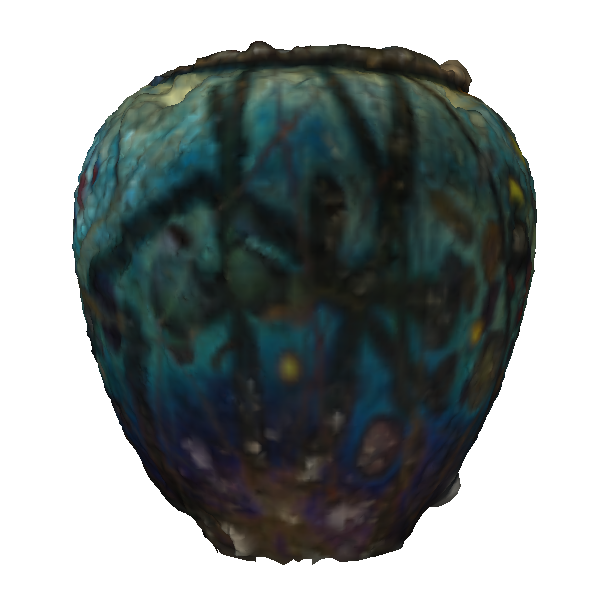
\includegraphics[width=0.33\textwidth]{interp/synth_data/vase/vase_mvs}\\
  ~ & MVS & ~\\
  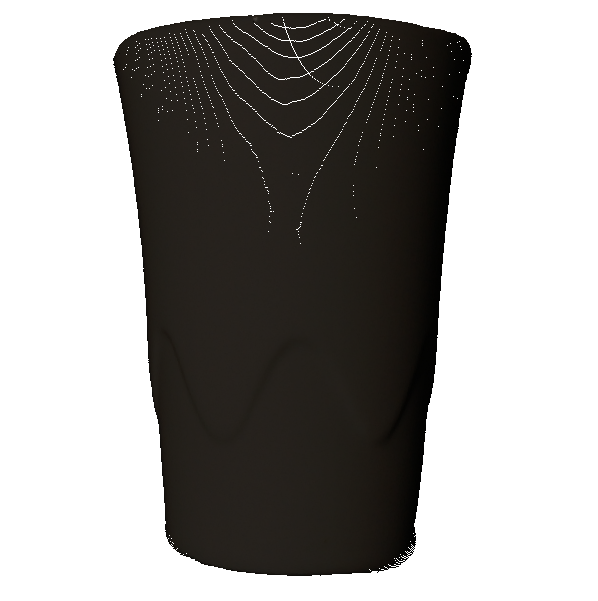
\includegraphics[width=0.33\textwidth]{interp/synth_data/cup/cup_ps}&
  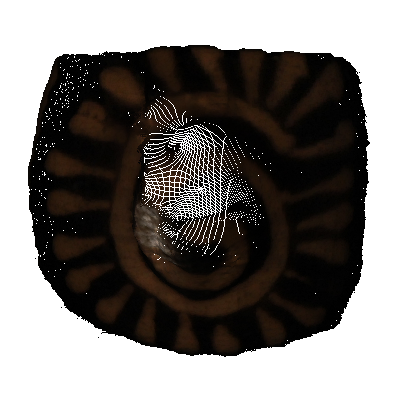
\includegraphics[width=0.33\textwidth]{interp/synth_data/pot/pot_ps}&
  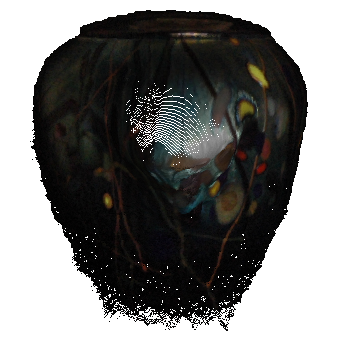
\includegraphics[width=0.33\textwidth]{interp/synth_data/vase/vase_ps}\\
  ~ & PS & ~\\
  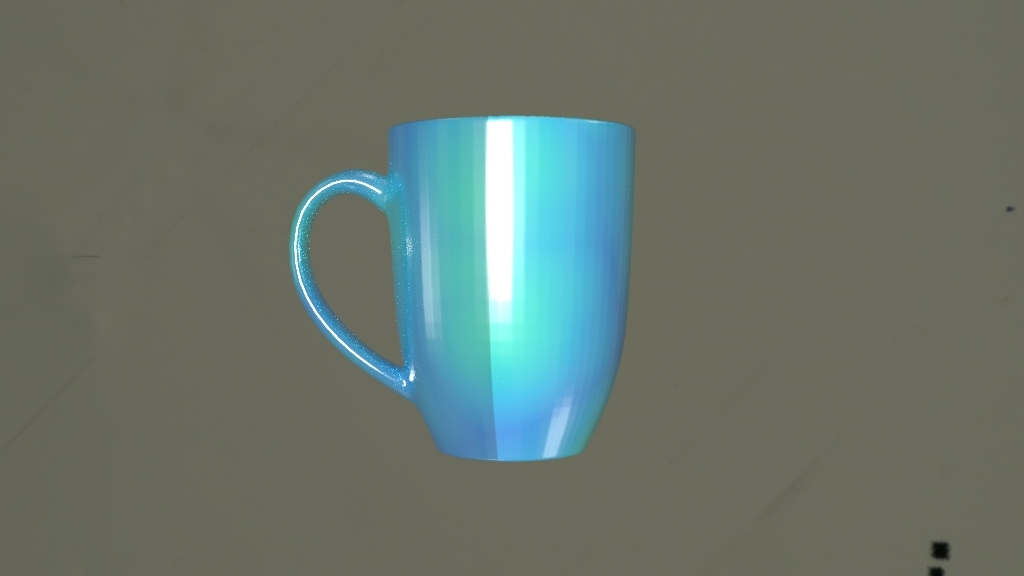
\includegraphics[width=0.33\textwidth]{interp/synth_data/cup/cup_sl}&
  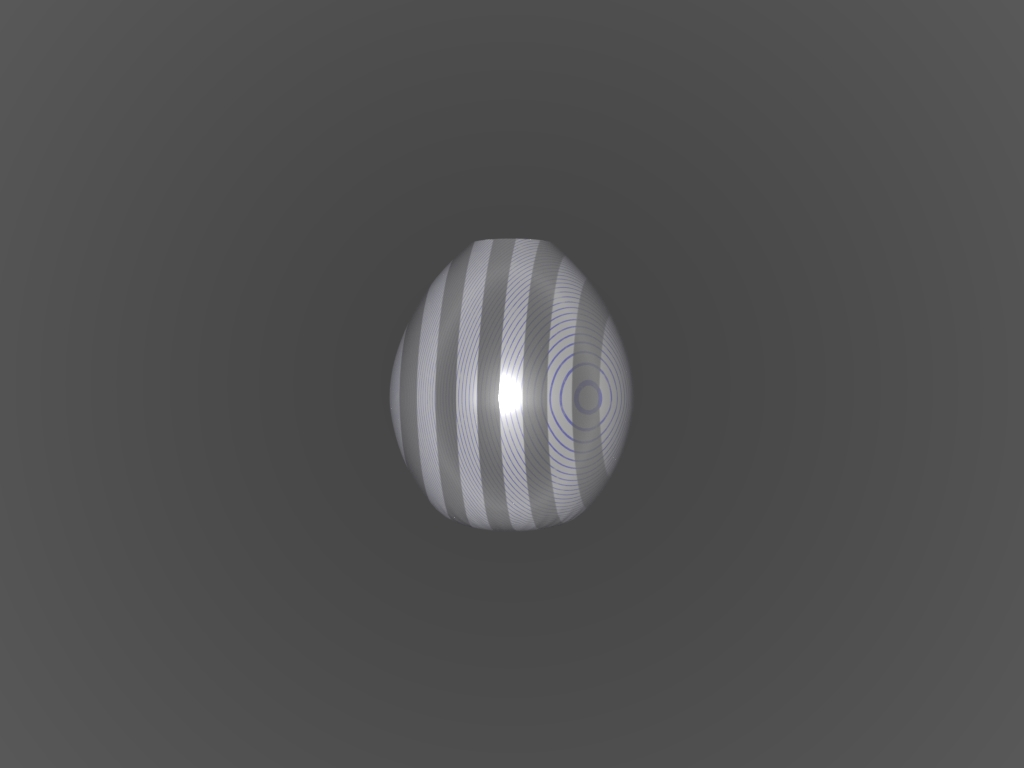
\includegraphics[width=0.33\textwidth]{interp/synth_data/pot/pot_sl}&
  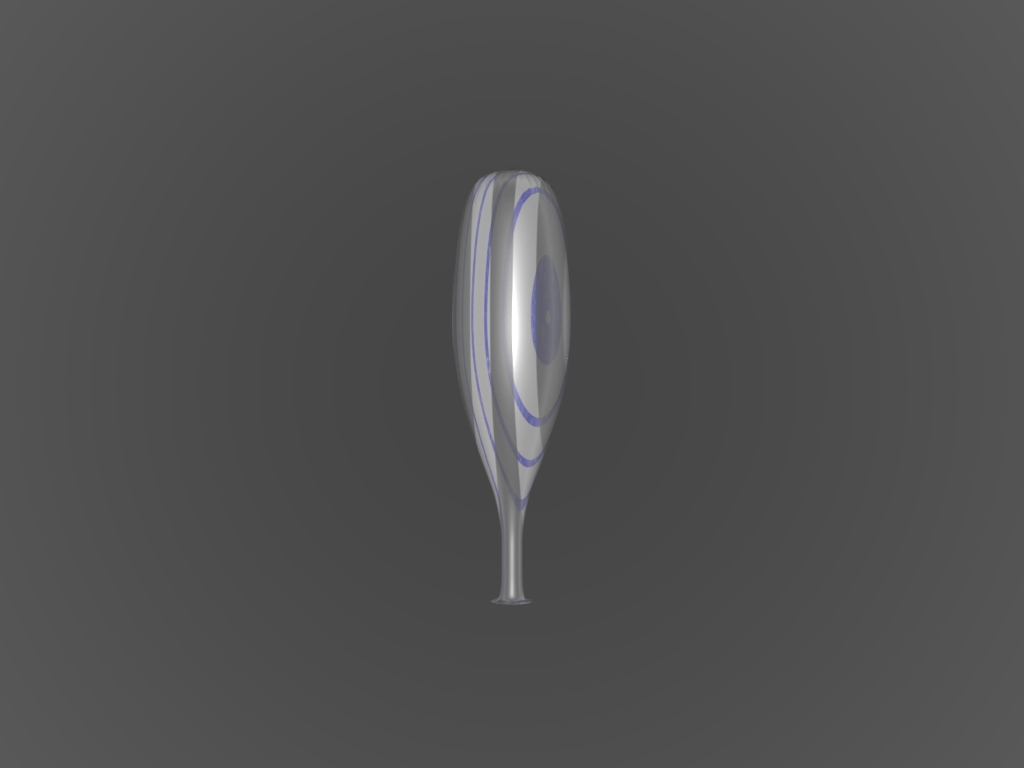
\includegraphics[width=0.33\textwidth]{interp/synth_data/vase/vase_sl}\\
  ~ & SL & ~\\
  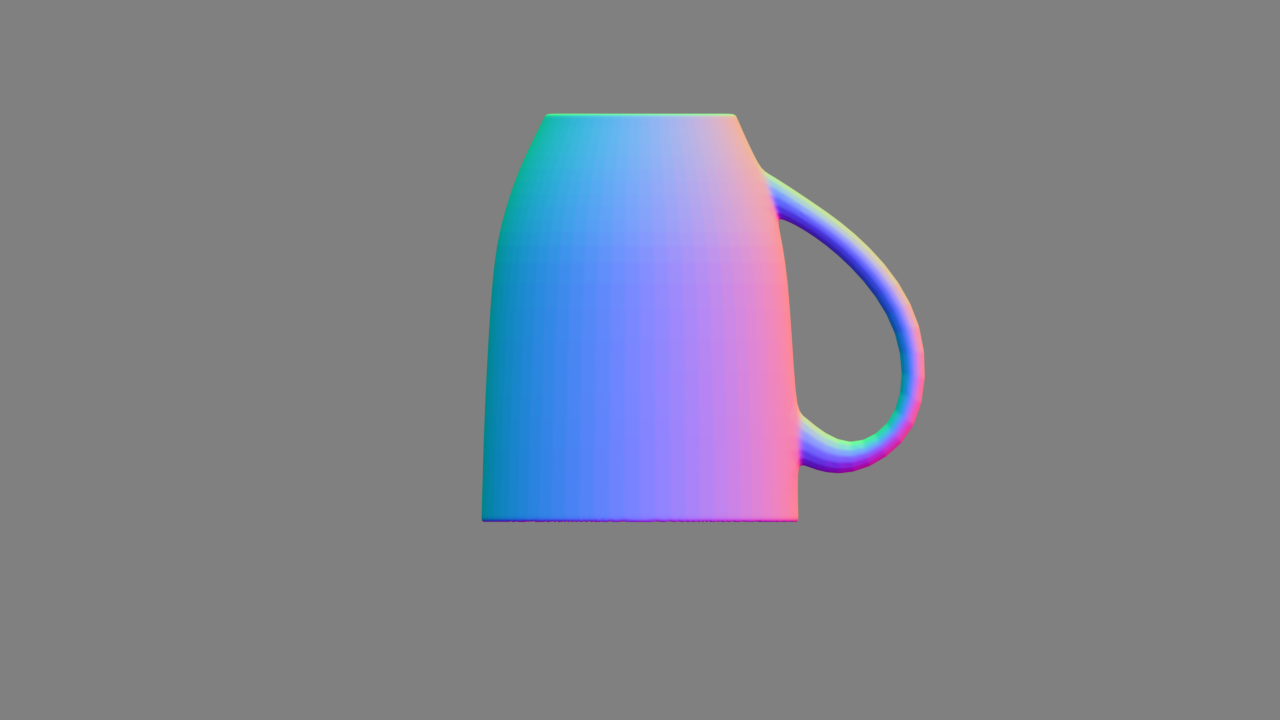
\includegraphics[width=0.33\textwidth]{interp/synth_data/cup/cup_gt}&
  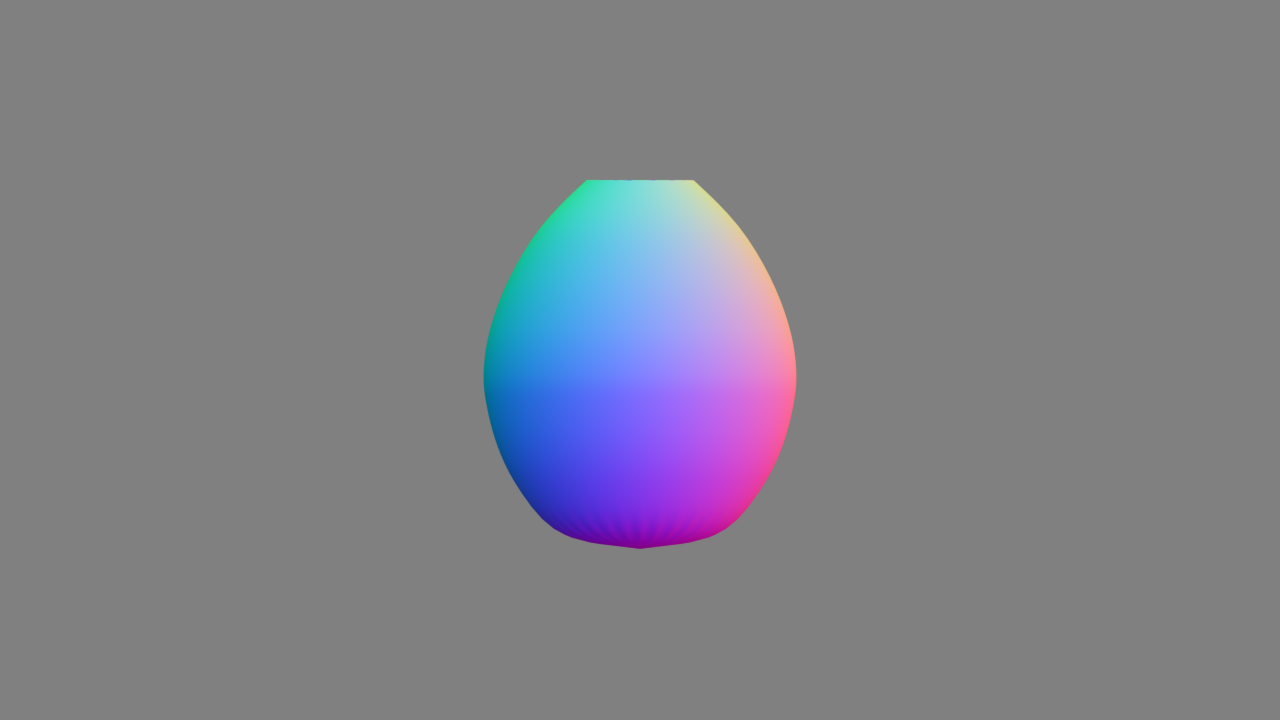
\includegraphics[width=0.33\textwidth]{interp/synth_data/pot/pot_gt}&
  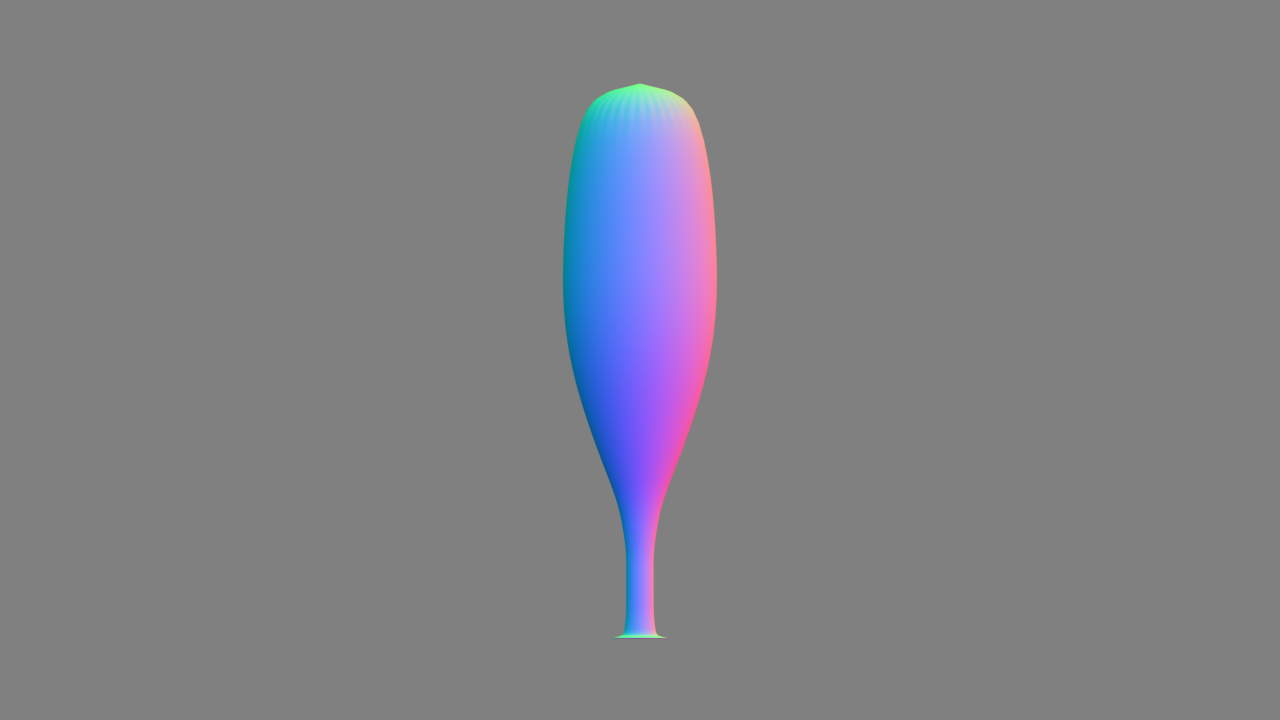
\includegraphics[width=0.33\textwidth]{interp/synth_data/vase/vase_gt}\\
  ~ & Normal groundtruth & ~\\
\end{tabular}
\caption{The synthetic datasets and groundtruth for the evaluation}
\label{fig:synth_data}
\end{figure}

Now we show both the quantitative results and qualitative results of the test objects, and see if the results is consistent with the techniques selected by our abstraction.

\textbf{Case 1} Both MVS and SL perform relatively well, but we can see that it has a bigger impact on the completeness, and less of an impact on the accuracy of MVS. This is consistent to the results shown in Table~\ref{tab:prop_list} (a). If it weren't for this abstraction, it would be hard to imagine that MVS actually works decently with relatively low textured surface. PS performs poorly as suggested by the abstraction, see Figure~\ref{fig:test_results_00}.

\begin{figure}[h!]
\centering
\begin{tabular}{ccccc}
  Quantitative results & ~ & Qualitative results & ~\\
  \includegraphics[width=2cm]{interp/synth_data/cup/cup_02020205}&
  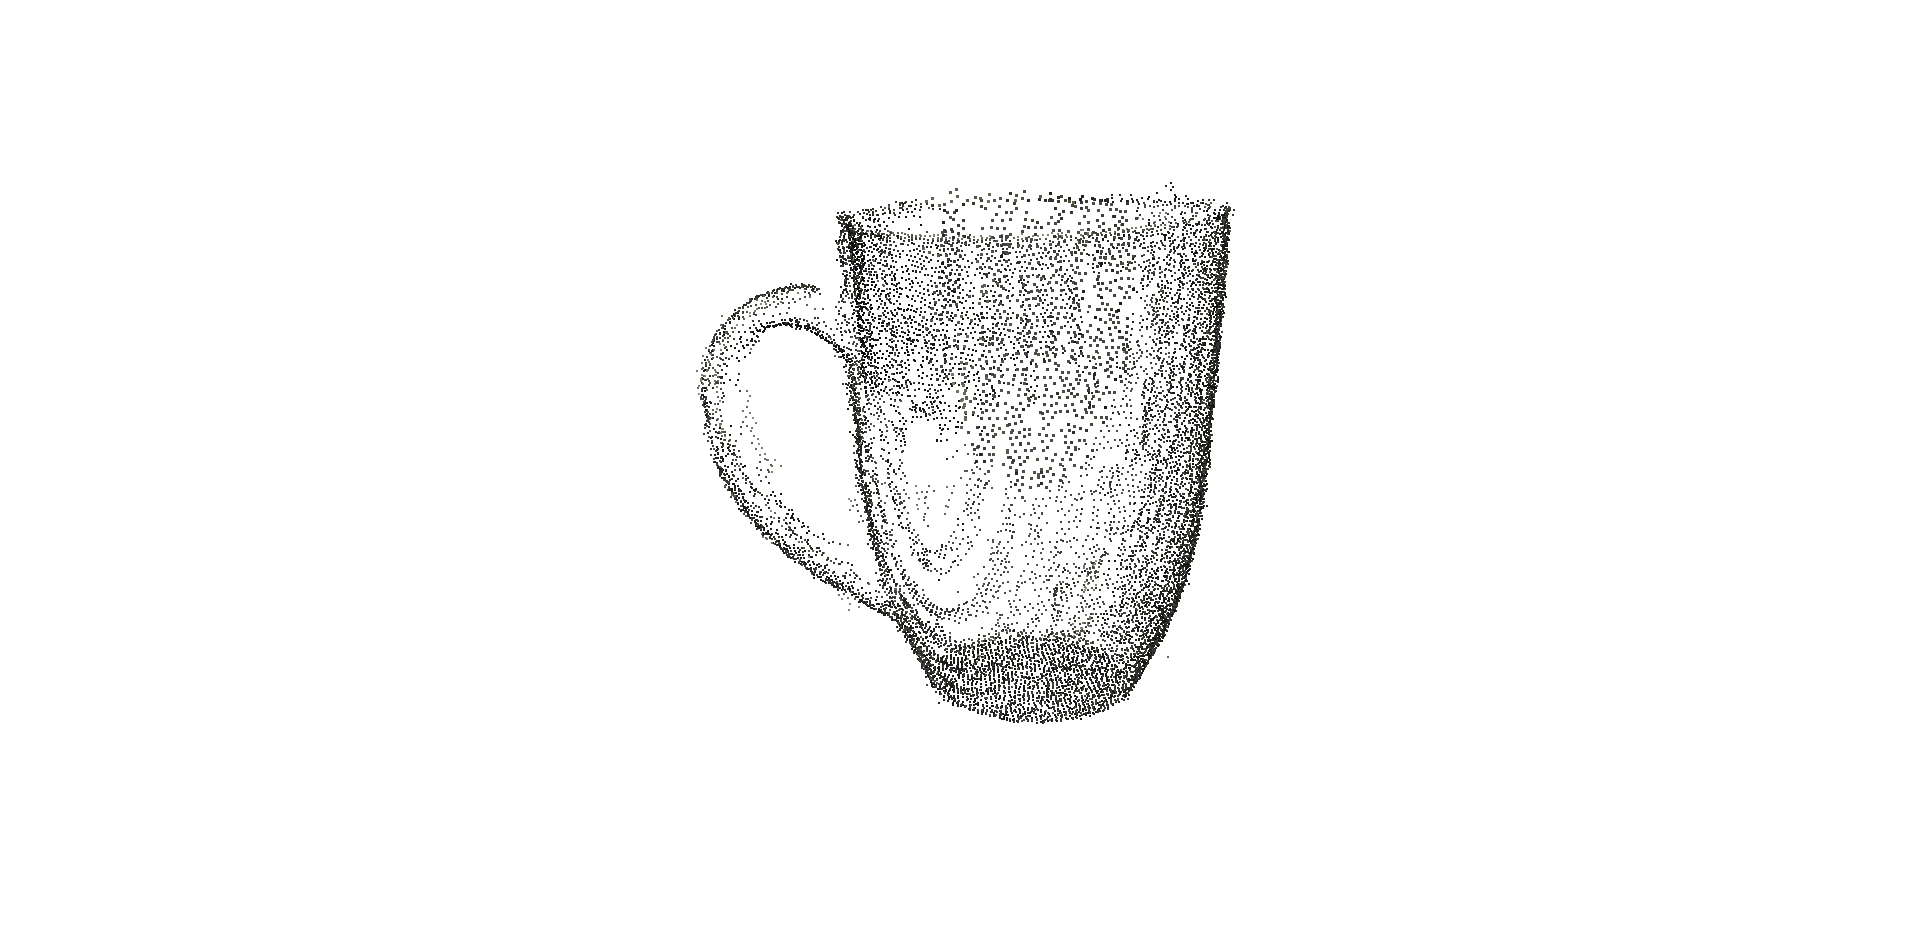
\includegraphics[width=2cm]{interp/synth_data/cup/cup_mvs_02020205.png}&
  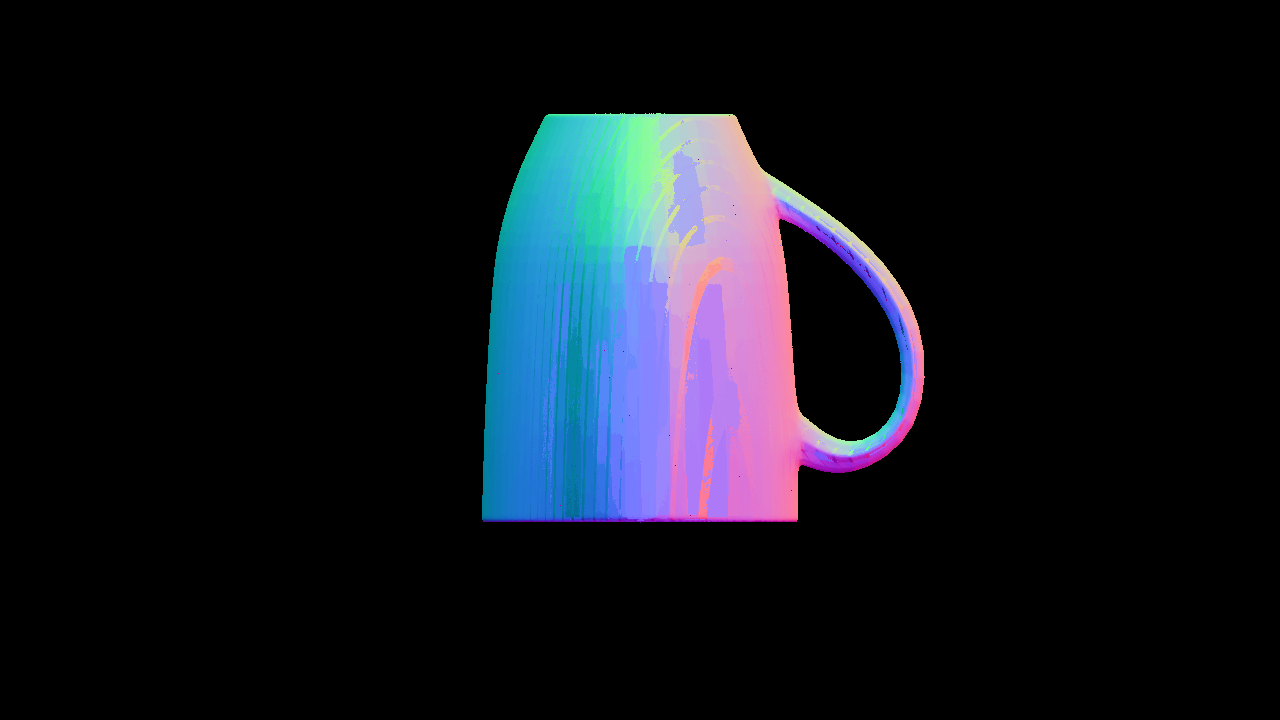
\includegraphics[width=2cm]{interp/synth_data/cup/cup_ps_02020205.png}&
  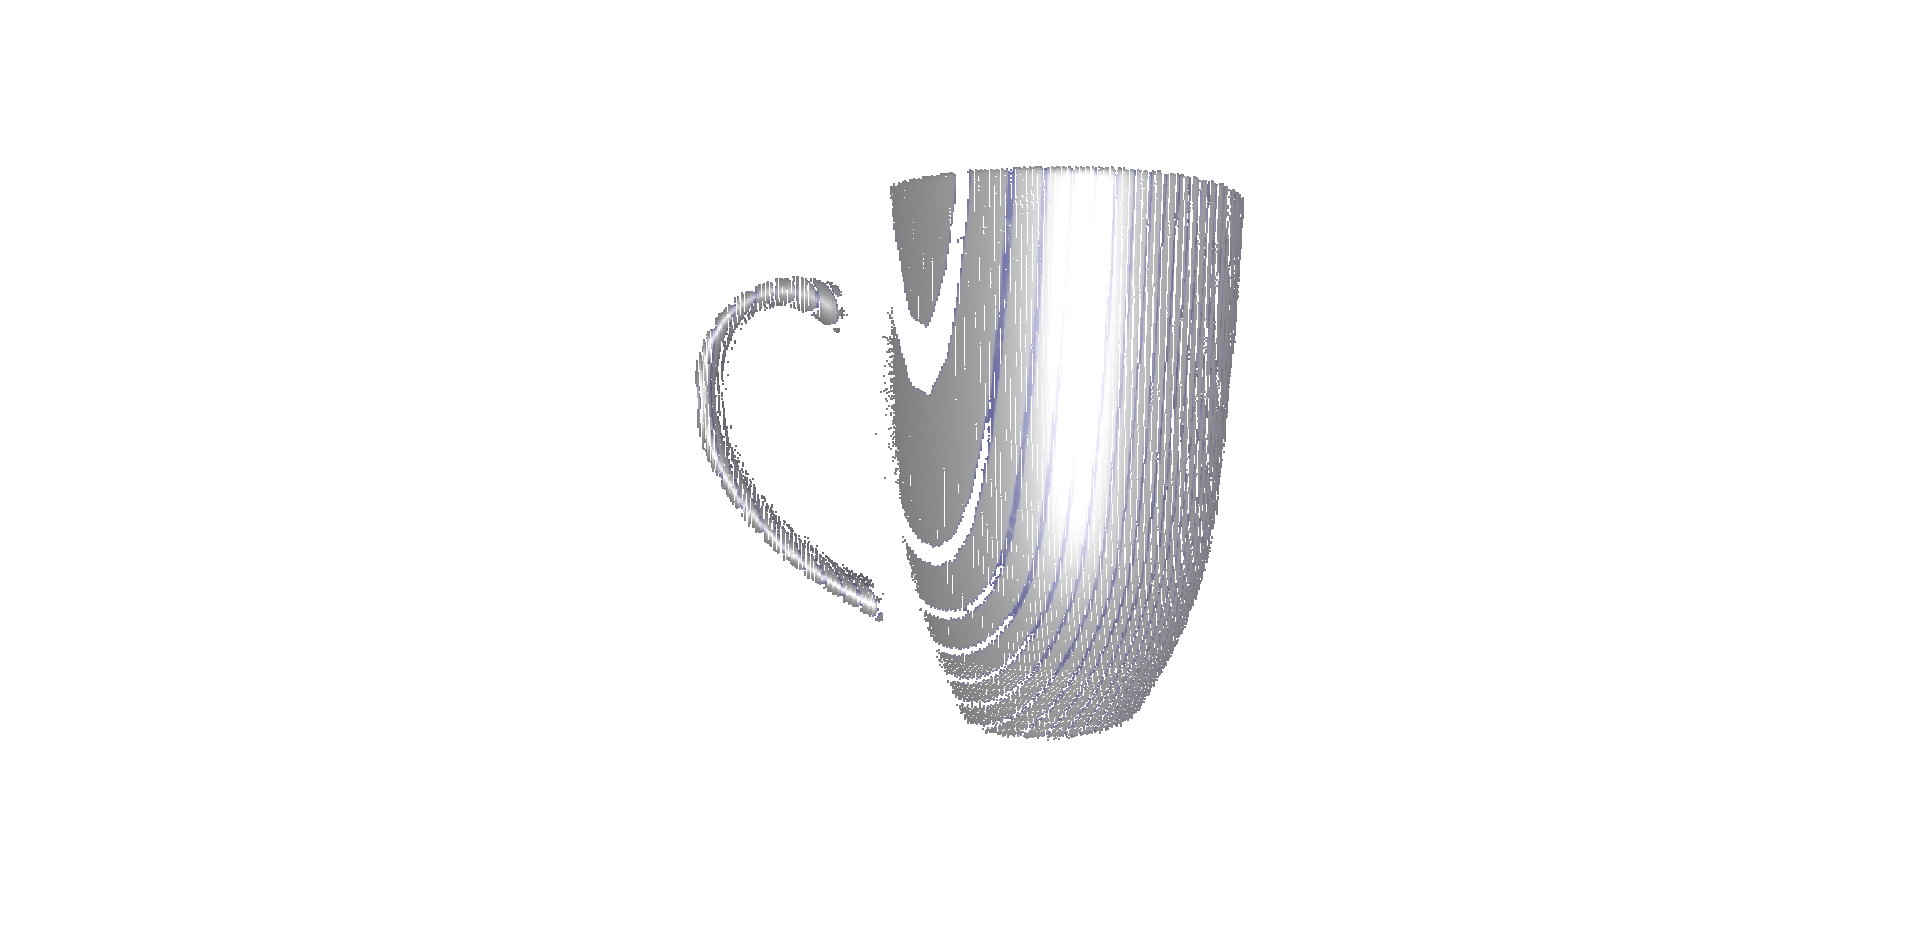
\includegraphics[width=2cm]{interp/synth_data/cup/cup_sl_02020205.png}\\
  \includegraphics[width=2cm]{interp/synth_data/pot/pot_02020205}&
  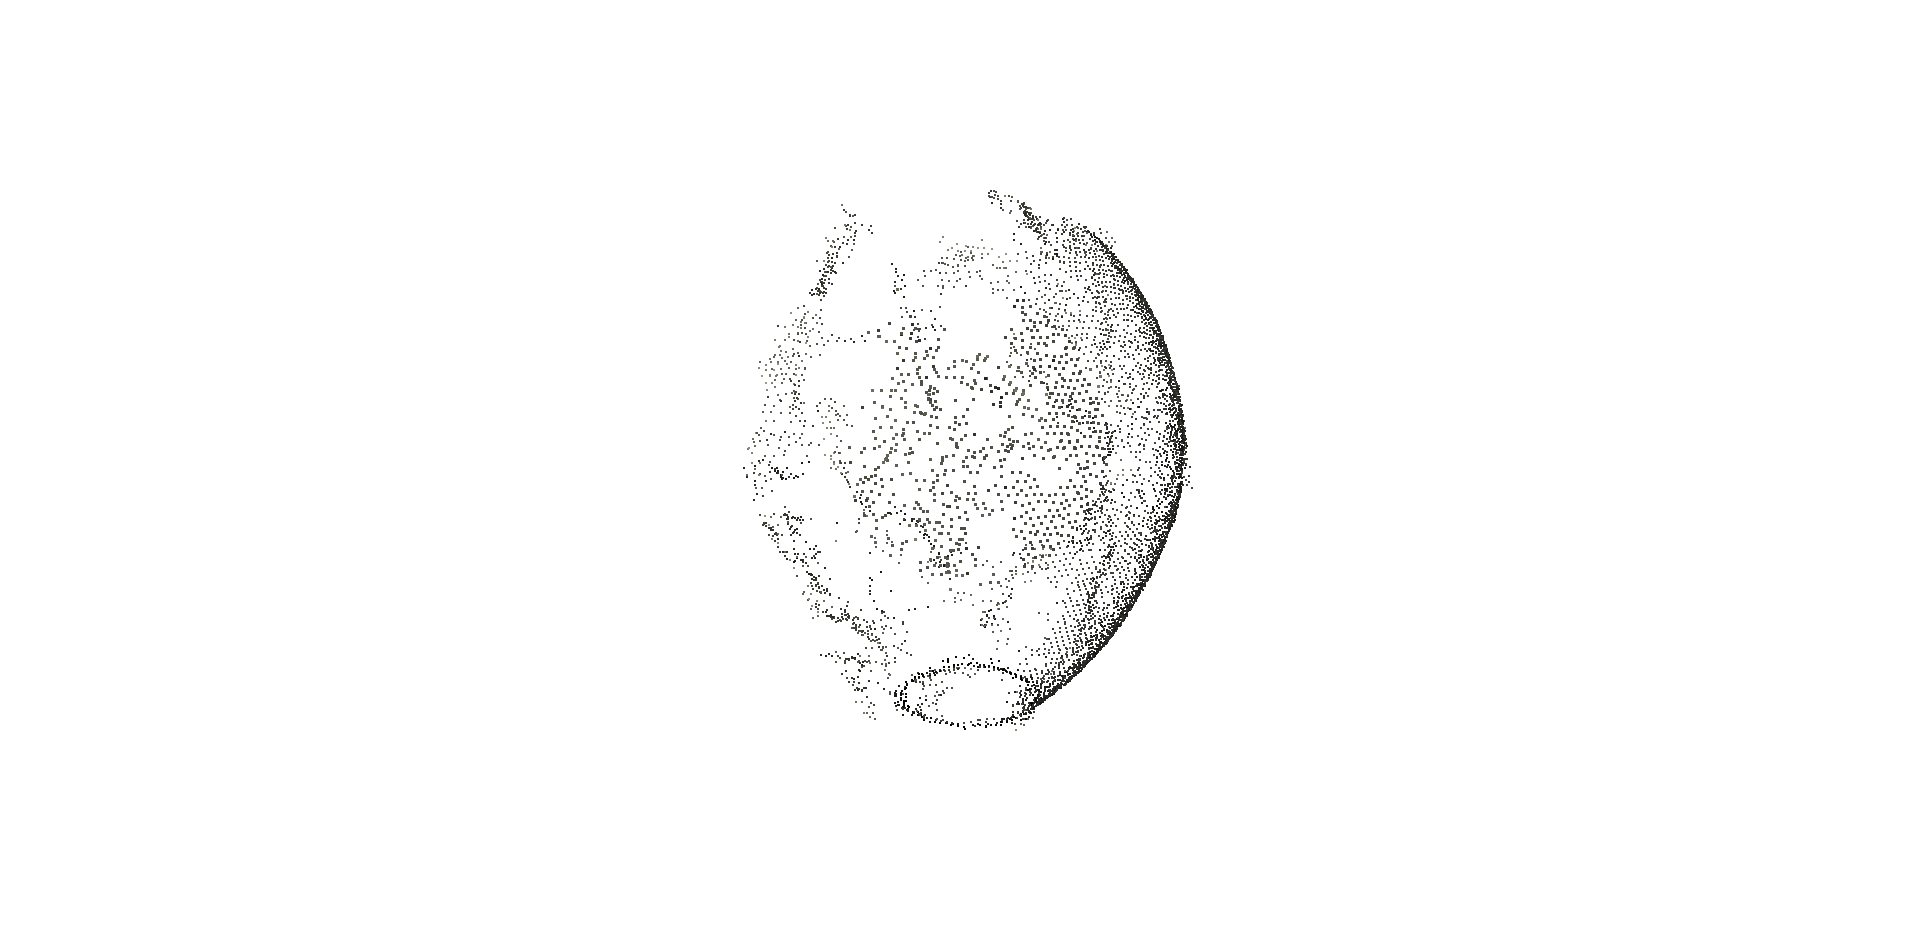
\includegraphics[width=2cm]{interp/synth_data/pot/pot_mvs_02020205.png}&
  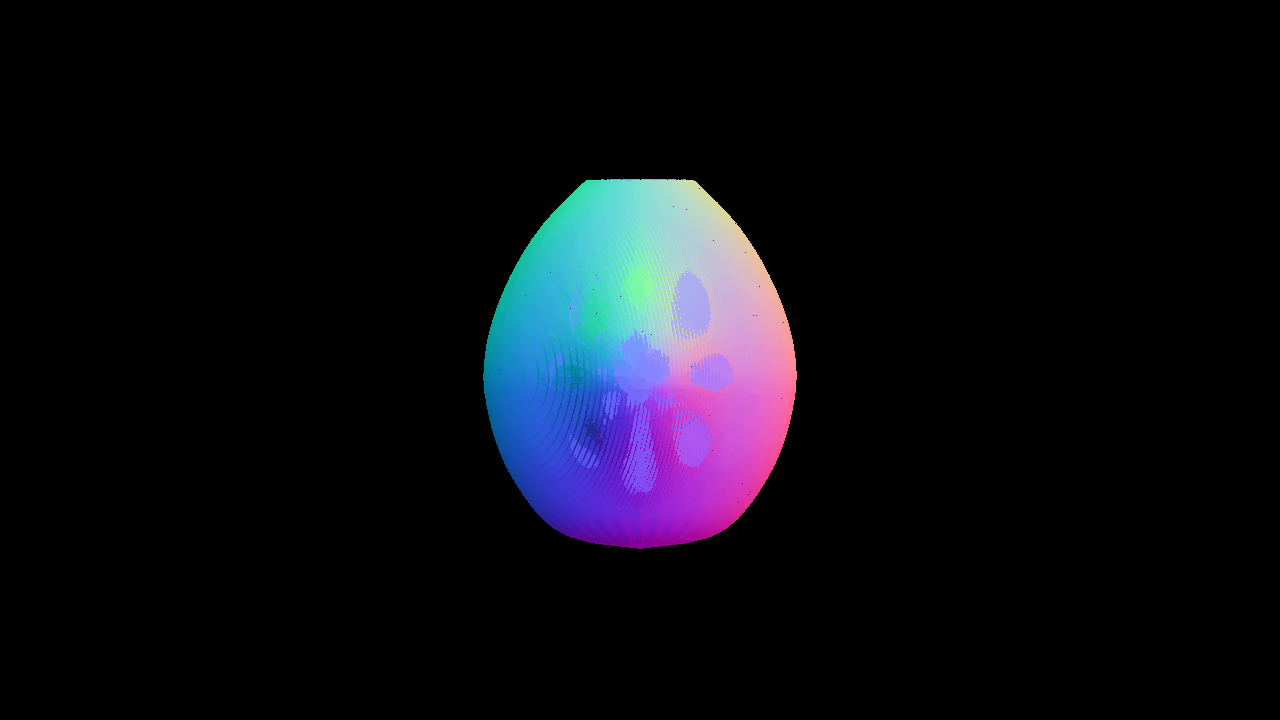
\includegraphics[width=2cm]{interp/synth_data/pot/pot_ps_02020205.png}&
  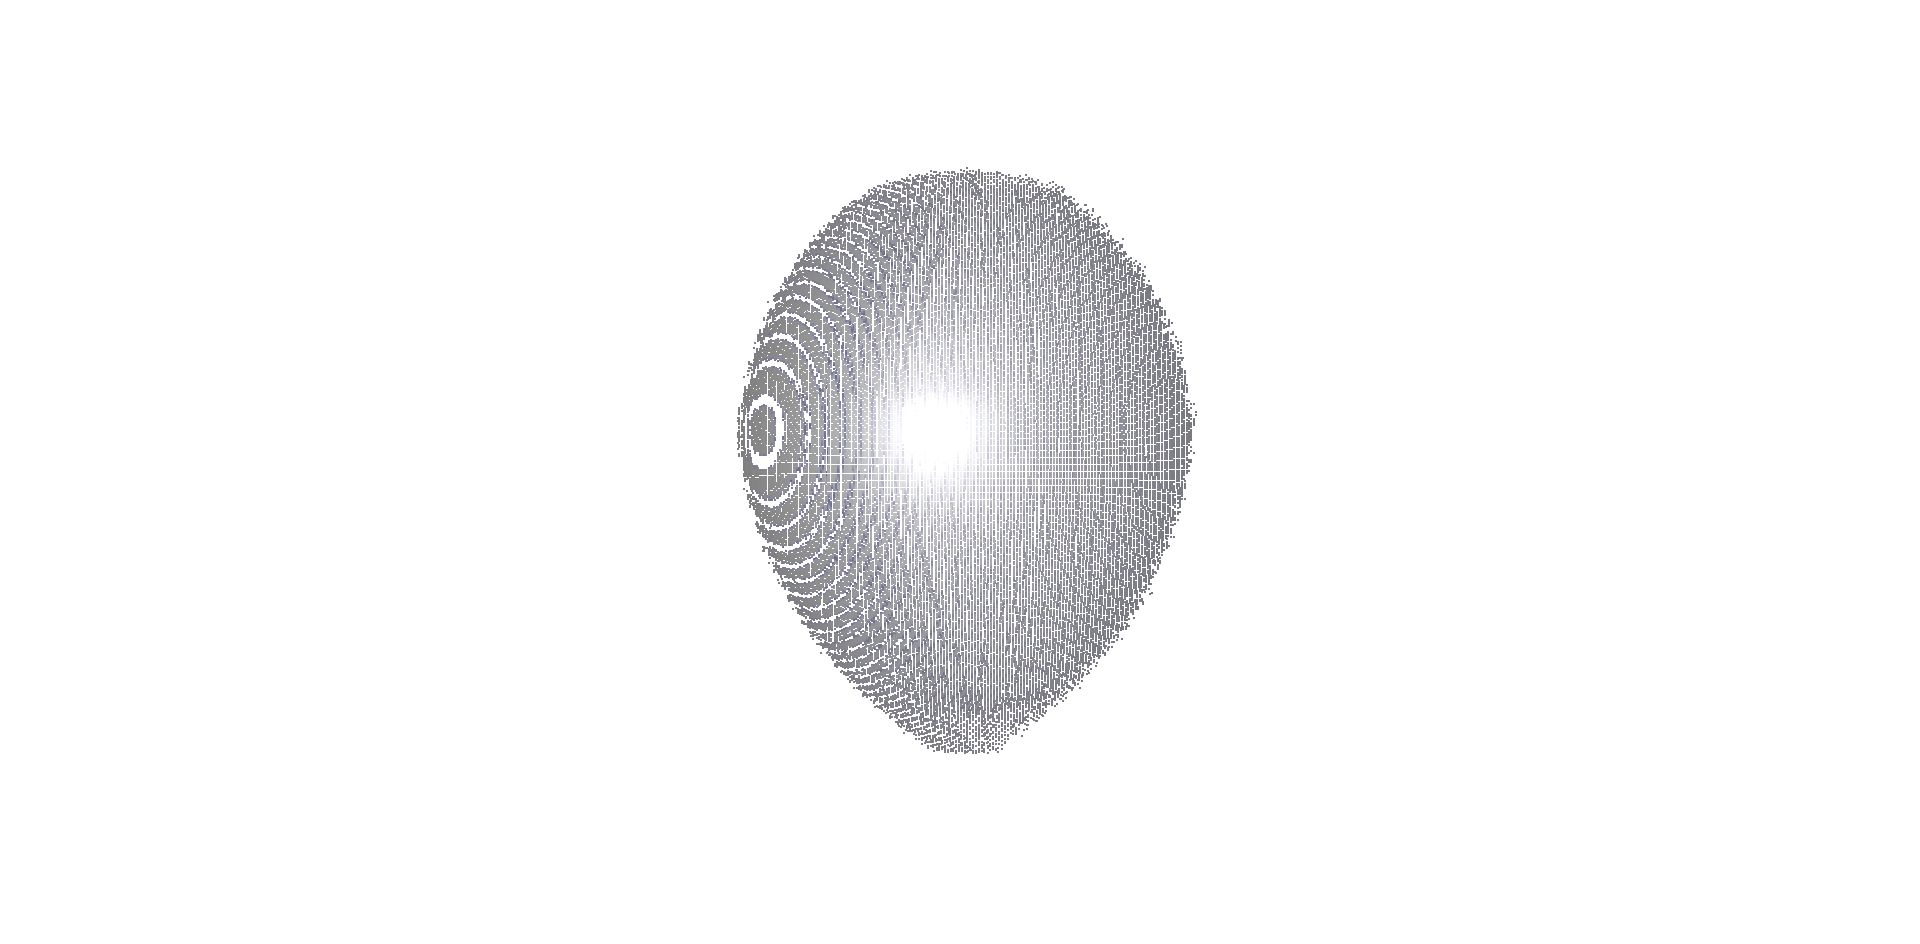
\includegraphics[width=2cm]{interp/synth_data/pot/pot_sl_02020205.png}\\
  \includegraphics[width=2cm]{interp/synth_data/vase/vase_02020205}&
  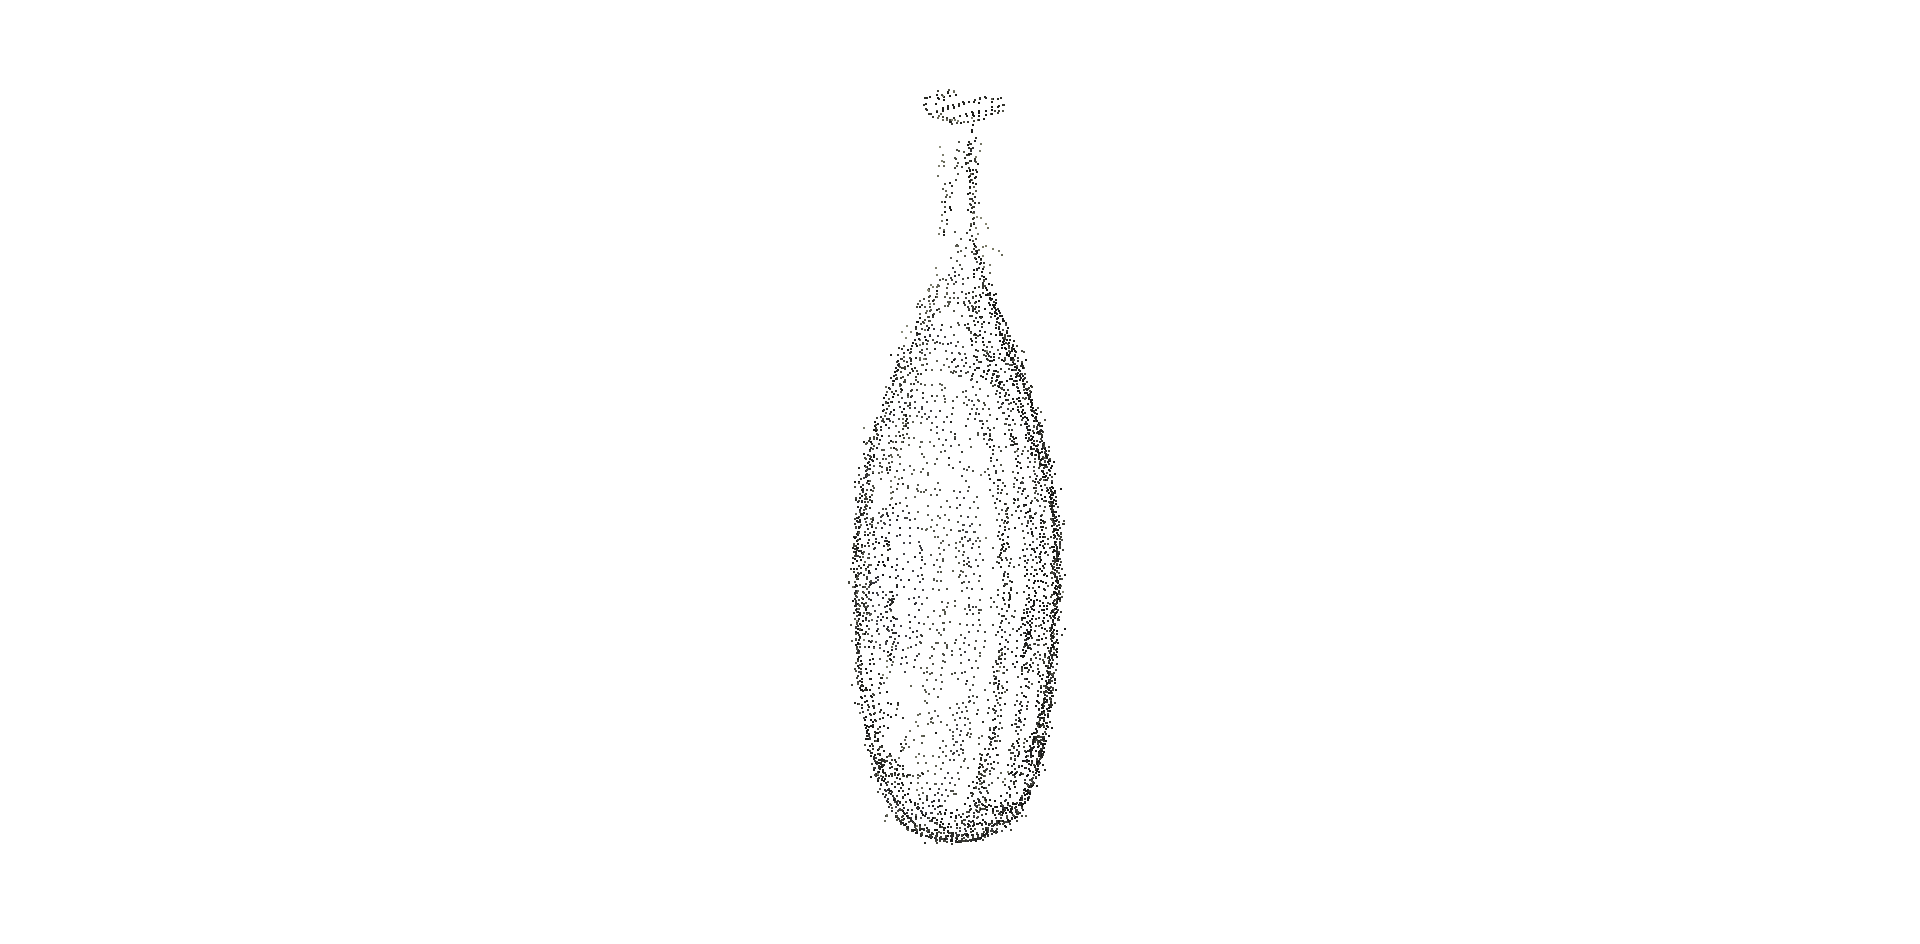
\includegraphics[width=2cm]{interp/synth_data/vase/vase_mvs_02020205.png}&
  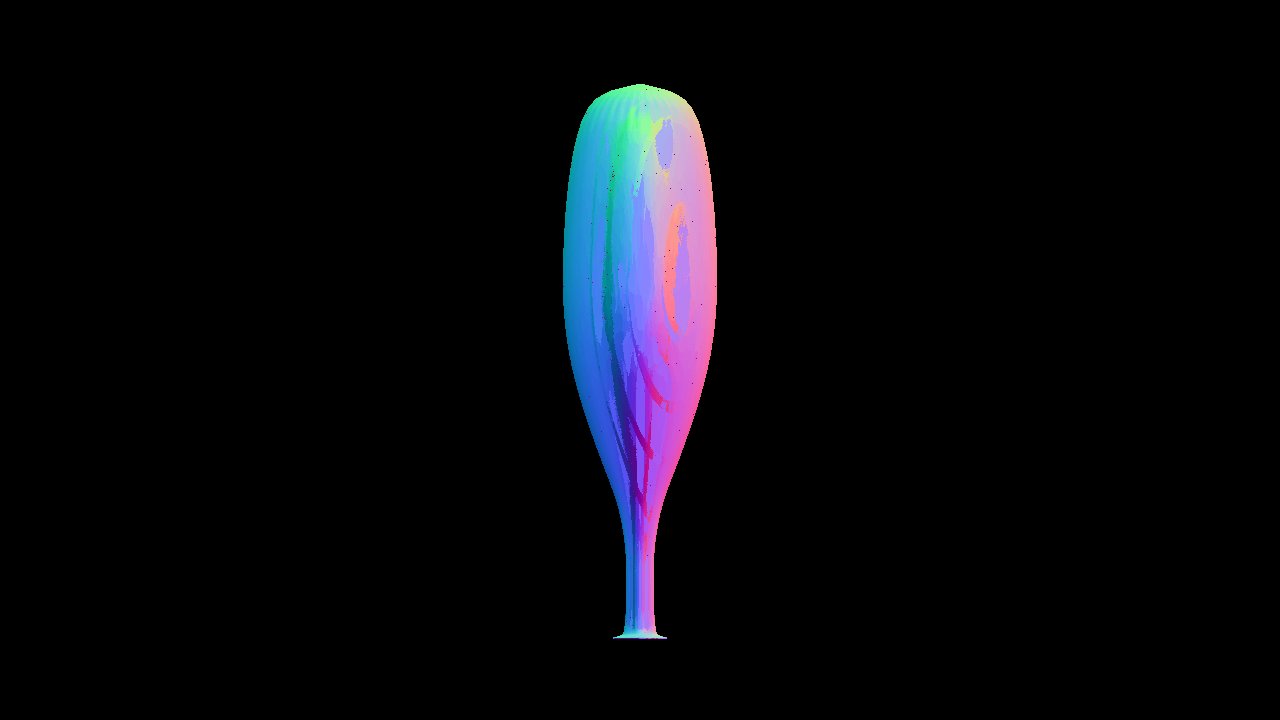
\includegraphics[width=2cm]{interp/synth_data/vase/vase_ps_02020205.png}&
  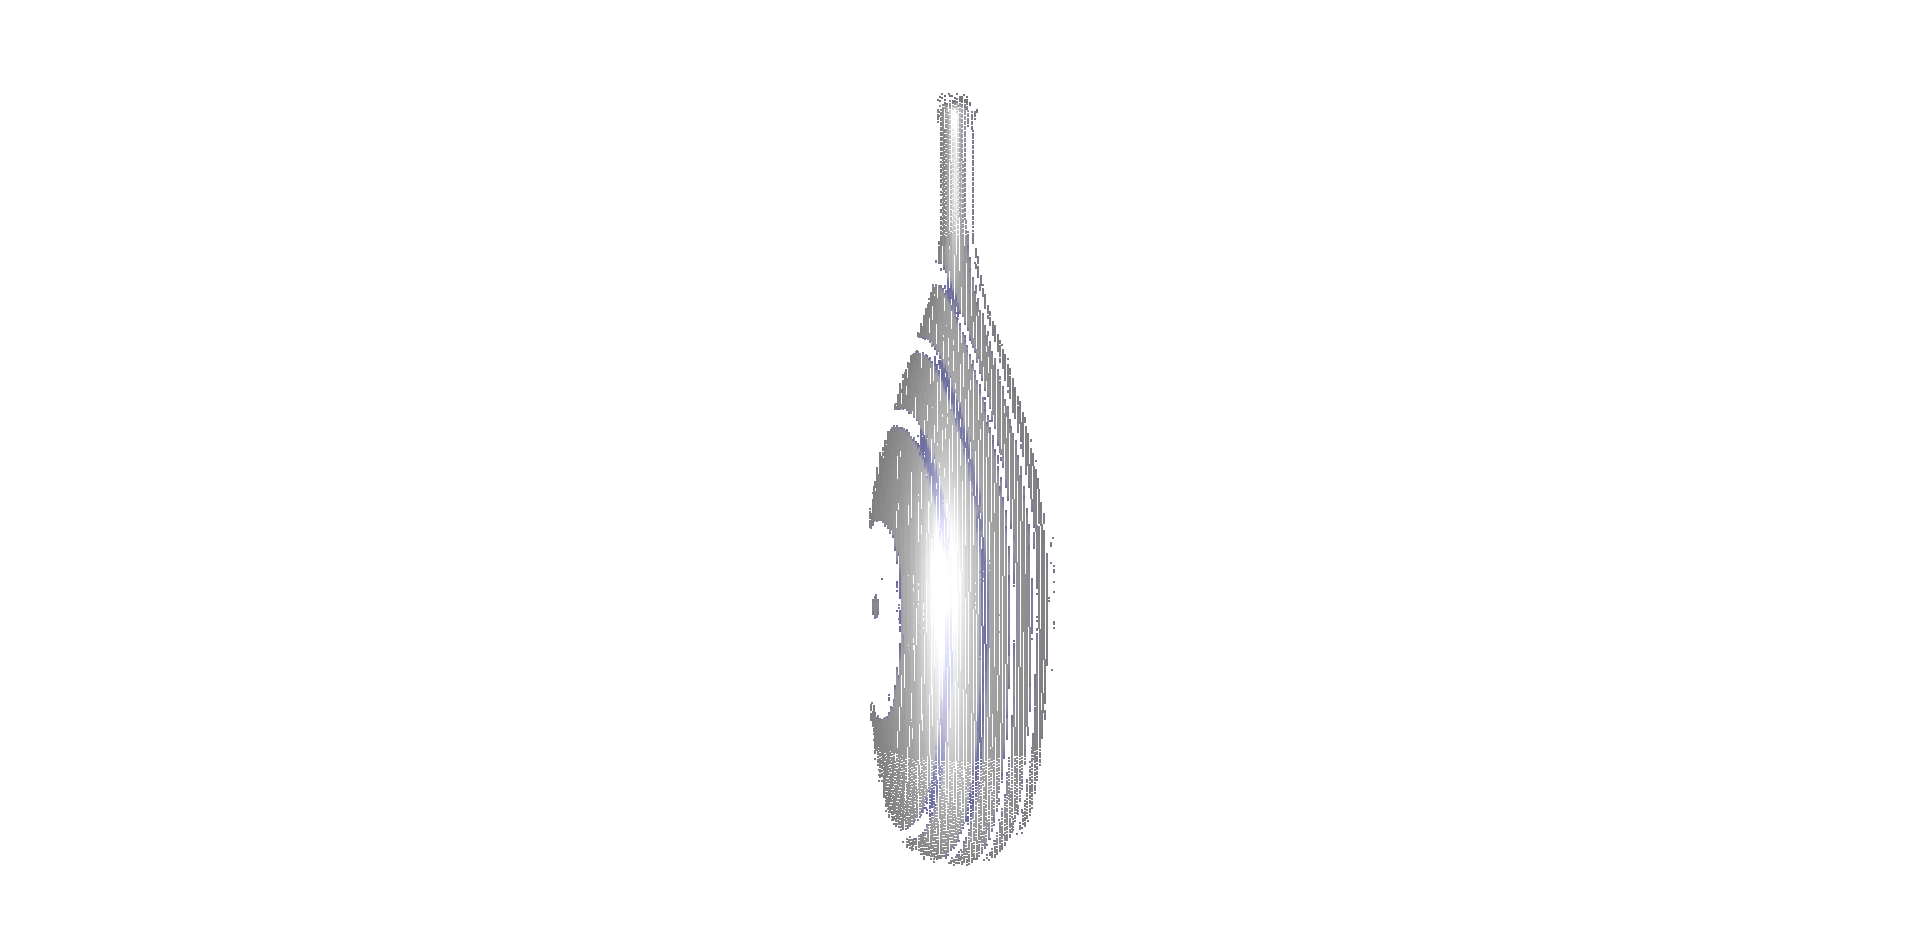
\includegraphics[width=2cm]{interp/synth_data/vase/vase_sl_02020205.png}\\
  ~& MVS & PS & SL\\
\end{tabular}
\caption{Property list: \{tex:0.2, alb:0.2, spec:0.2, rough: 0.5\}. The quantitative and qualitative performance of each technique on three test objects}
\label{fig:test_results_00}
\end{figure}

\textbf{Case 2} All three techniques perform well in this case, , see Figure~\ref{fig:test_results_01}, which is consistent to the result returned by the abstraction which is shown in Table~\ref{tab:prop_list} (b).

\begin{figure}[h!]
\centering
\begin{tabular}{ccccc}
  Quantitative results & ~ & Qualitative results & ~\\
  \includegraphics[width=2cm]{interp/synth_data/cup/cup_02080205}&
  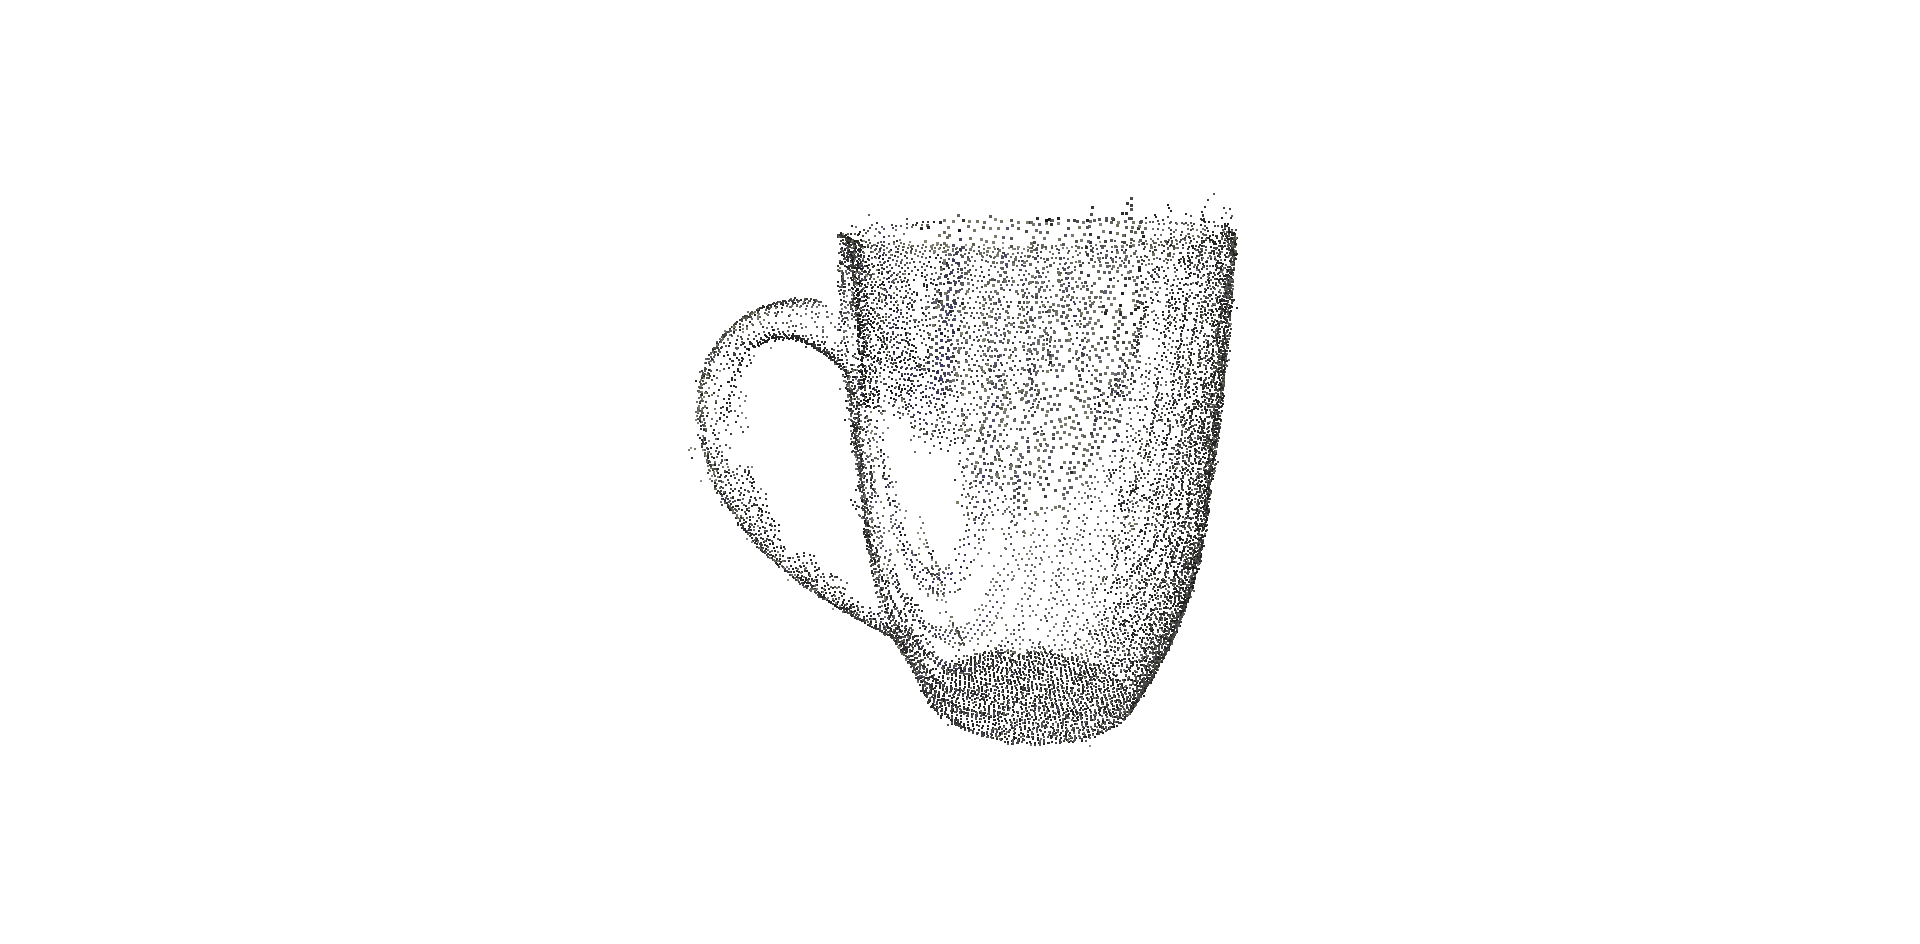
\includegraphics[width=2cm]{interp/synth_data/cup/cup_mvs_02080205.png}&
  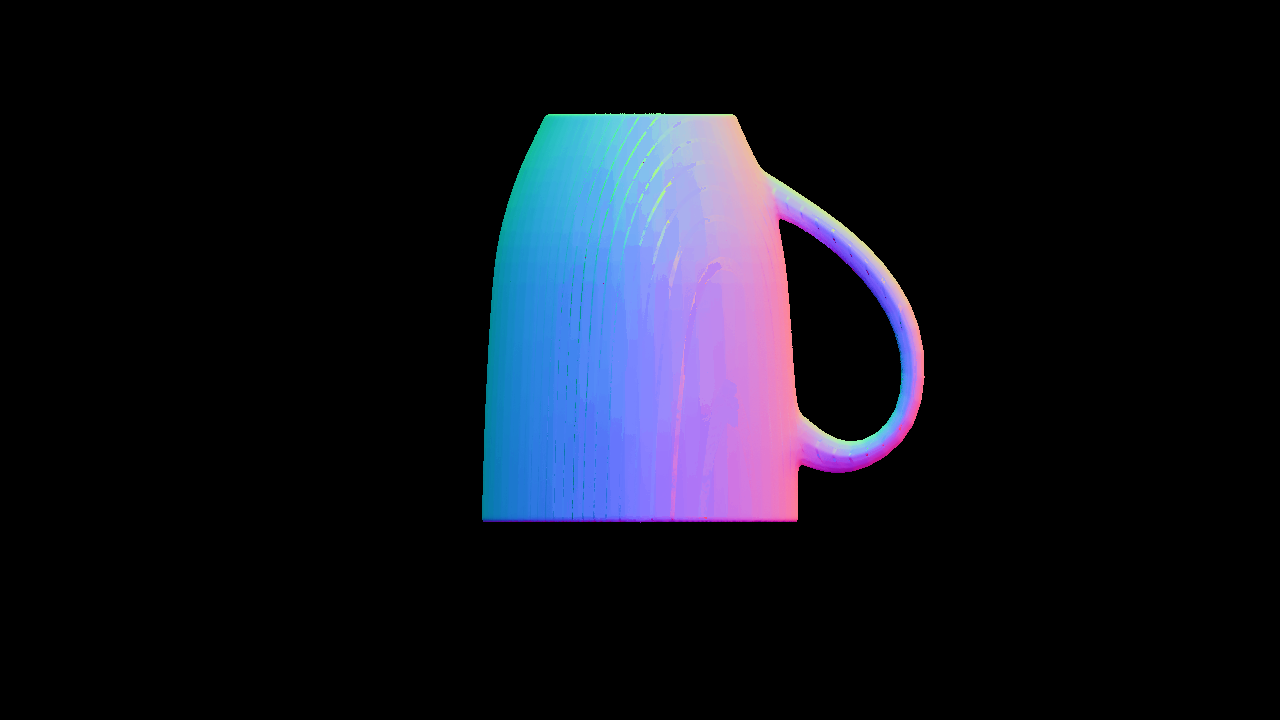
\includegraphics[width=2cm]{interp/synth_data/cup/cup_ps_02080205.png}&
  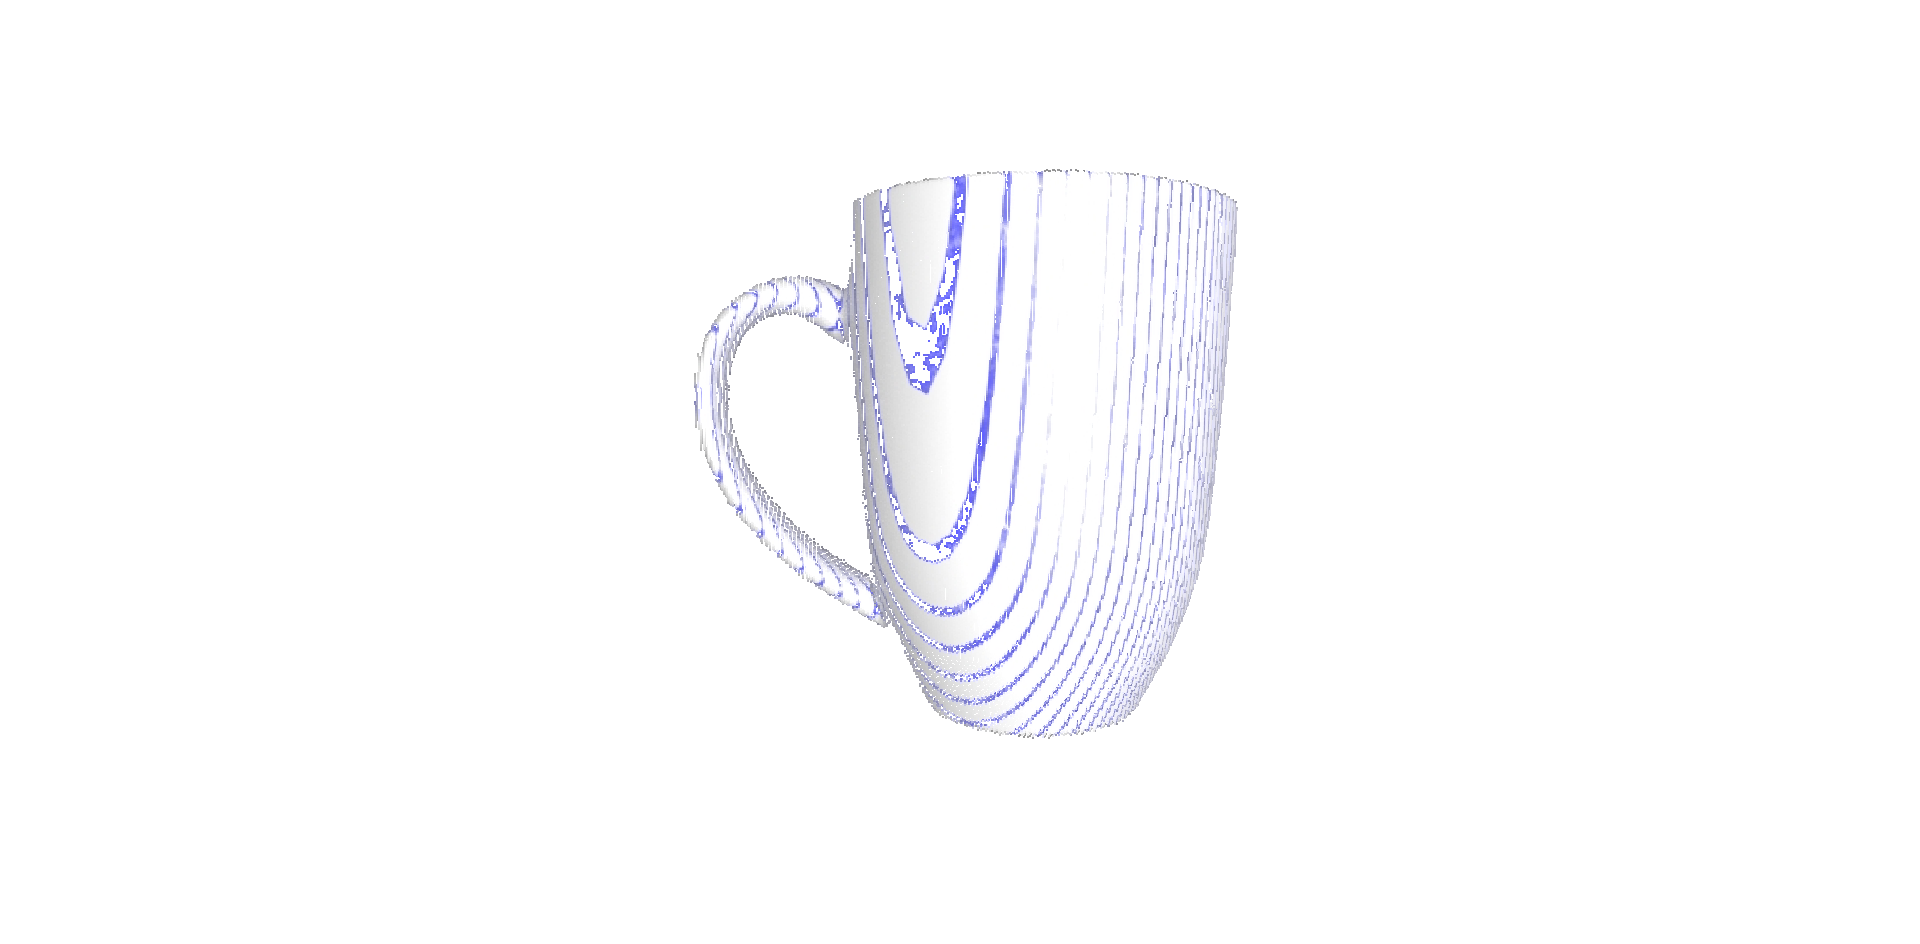
\includegraphics[width=2cm]{interp/synth_data/cup/cup_sl_02080205.png}\\
  \includegraphics[width=2cm]{interp/synth_data/pot/pot_02080205}&
  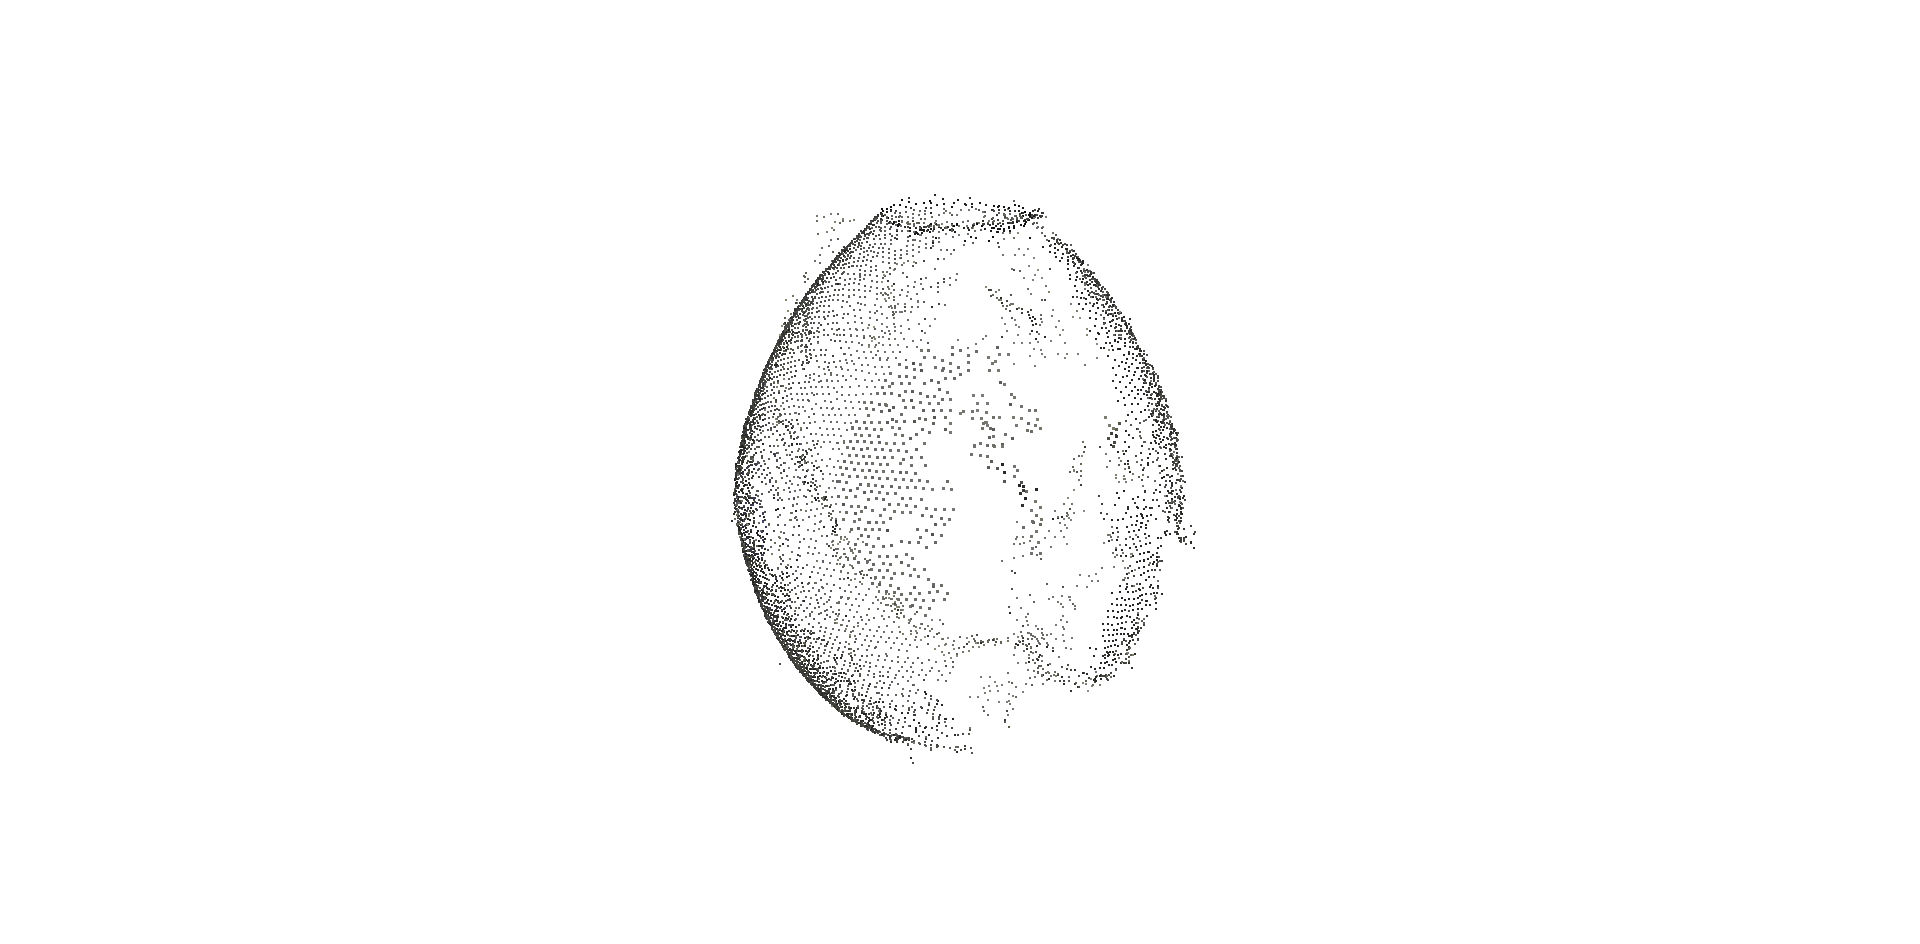
\includegraphics[width=2cm]{interp/synth_data/pot/pot_mvs_02080205.png}&
  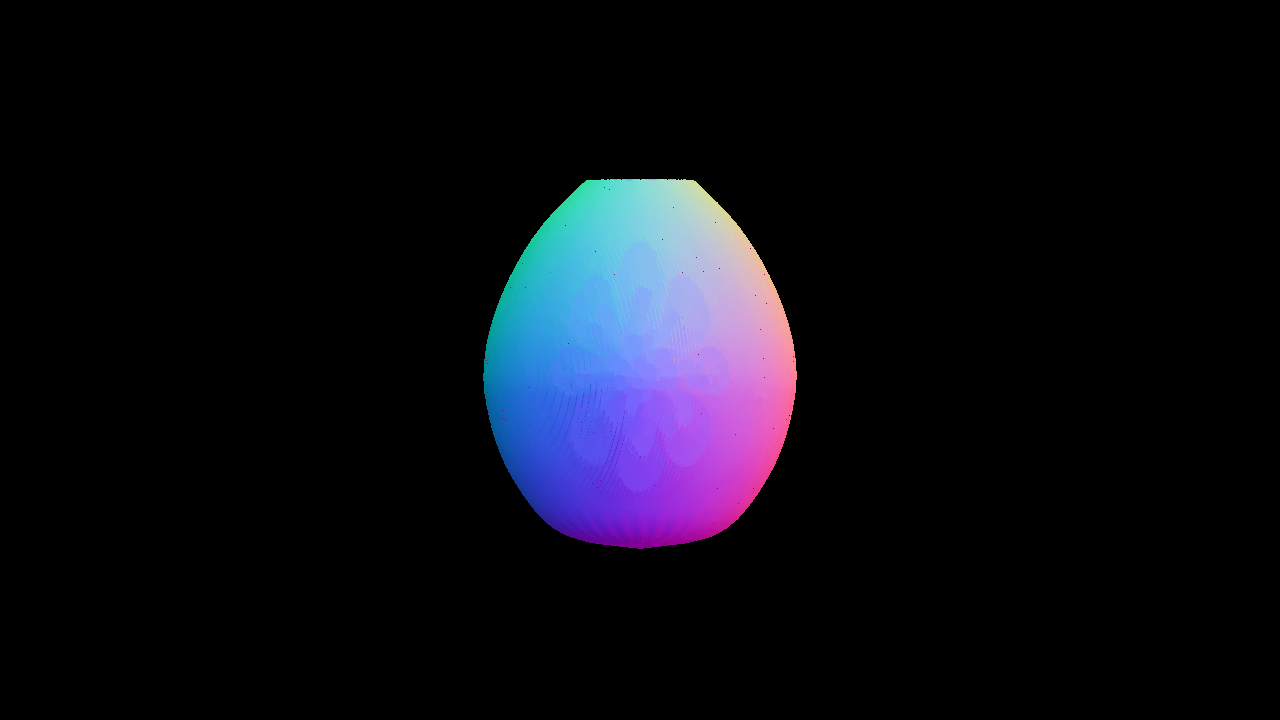
\includegraphics[width=2cm]{interp/synth_data/pot/pot_ps_02080205.png}&
  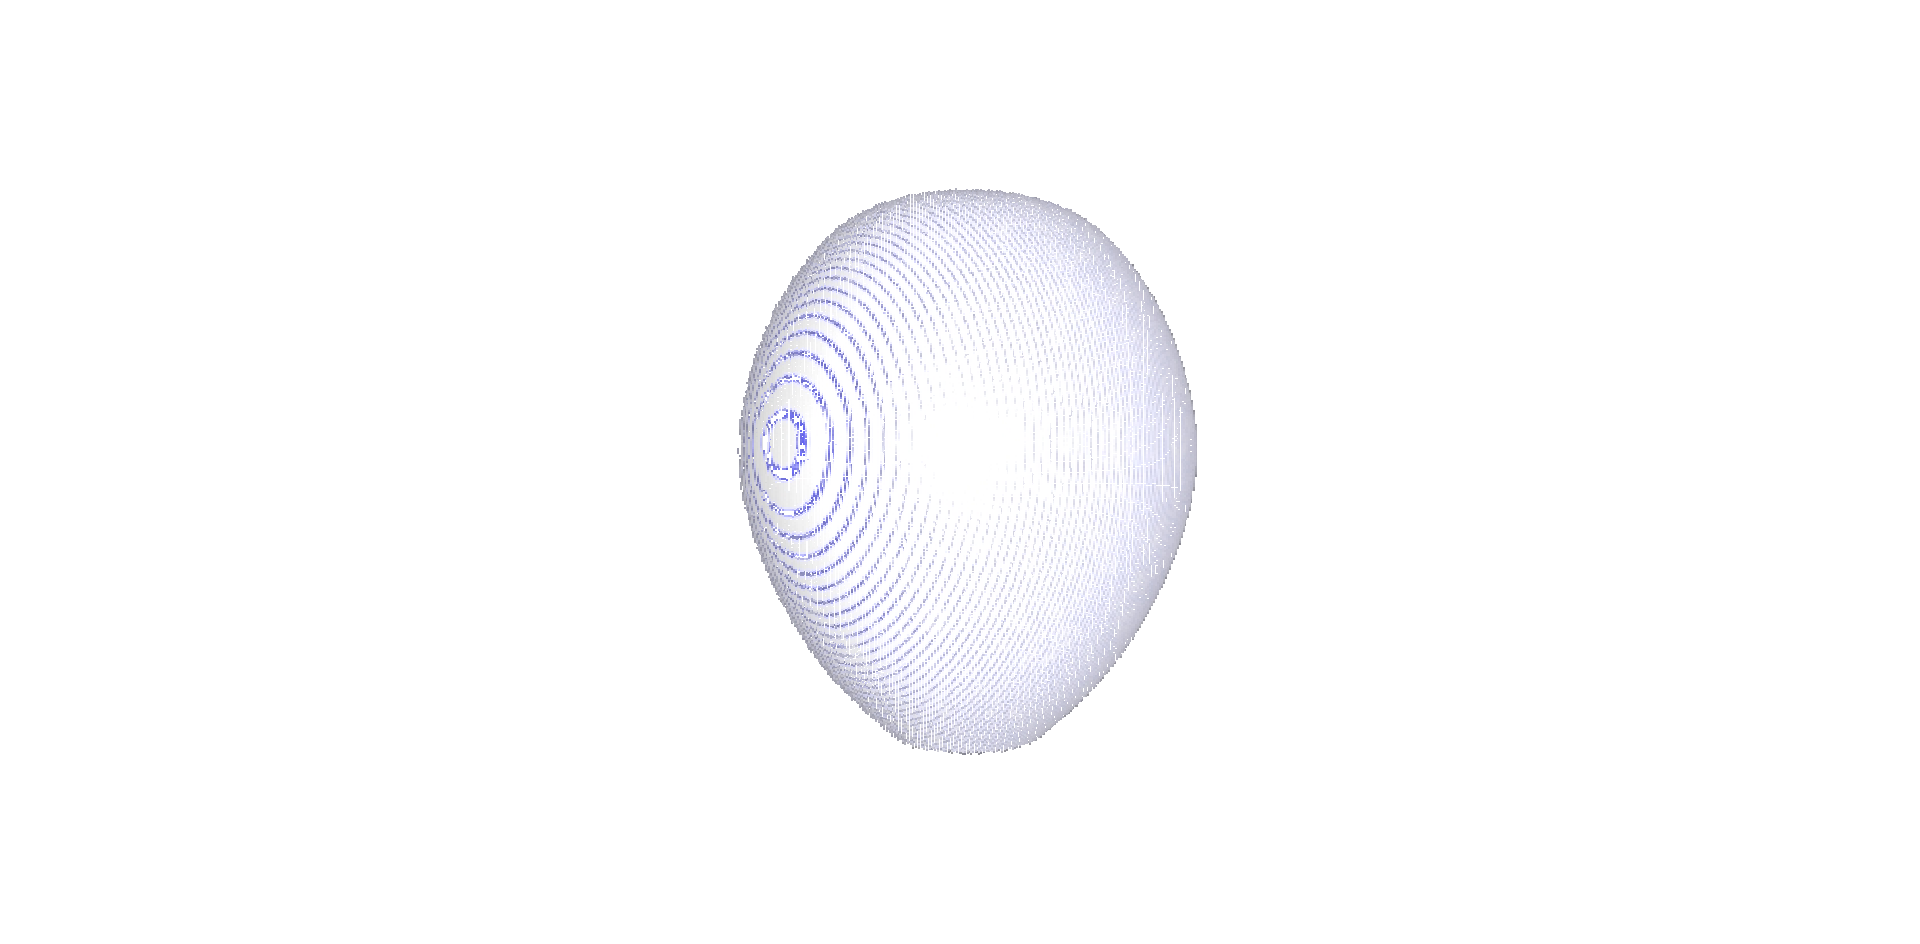
\includegraphics[width=2cm]{interp/synth_data/pot/pot_sl_02080205.png}\\
  \includegraphics[width=2cm]{interp/synth_data/vase/vase_02080205}&
  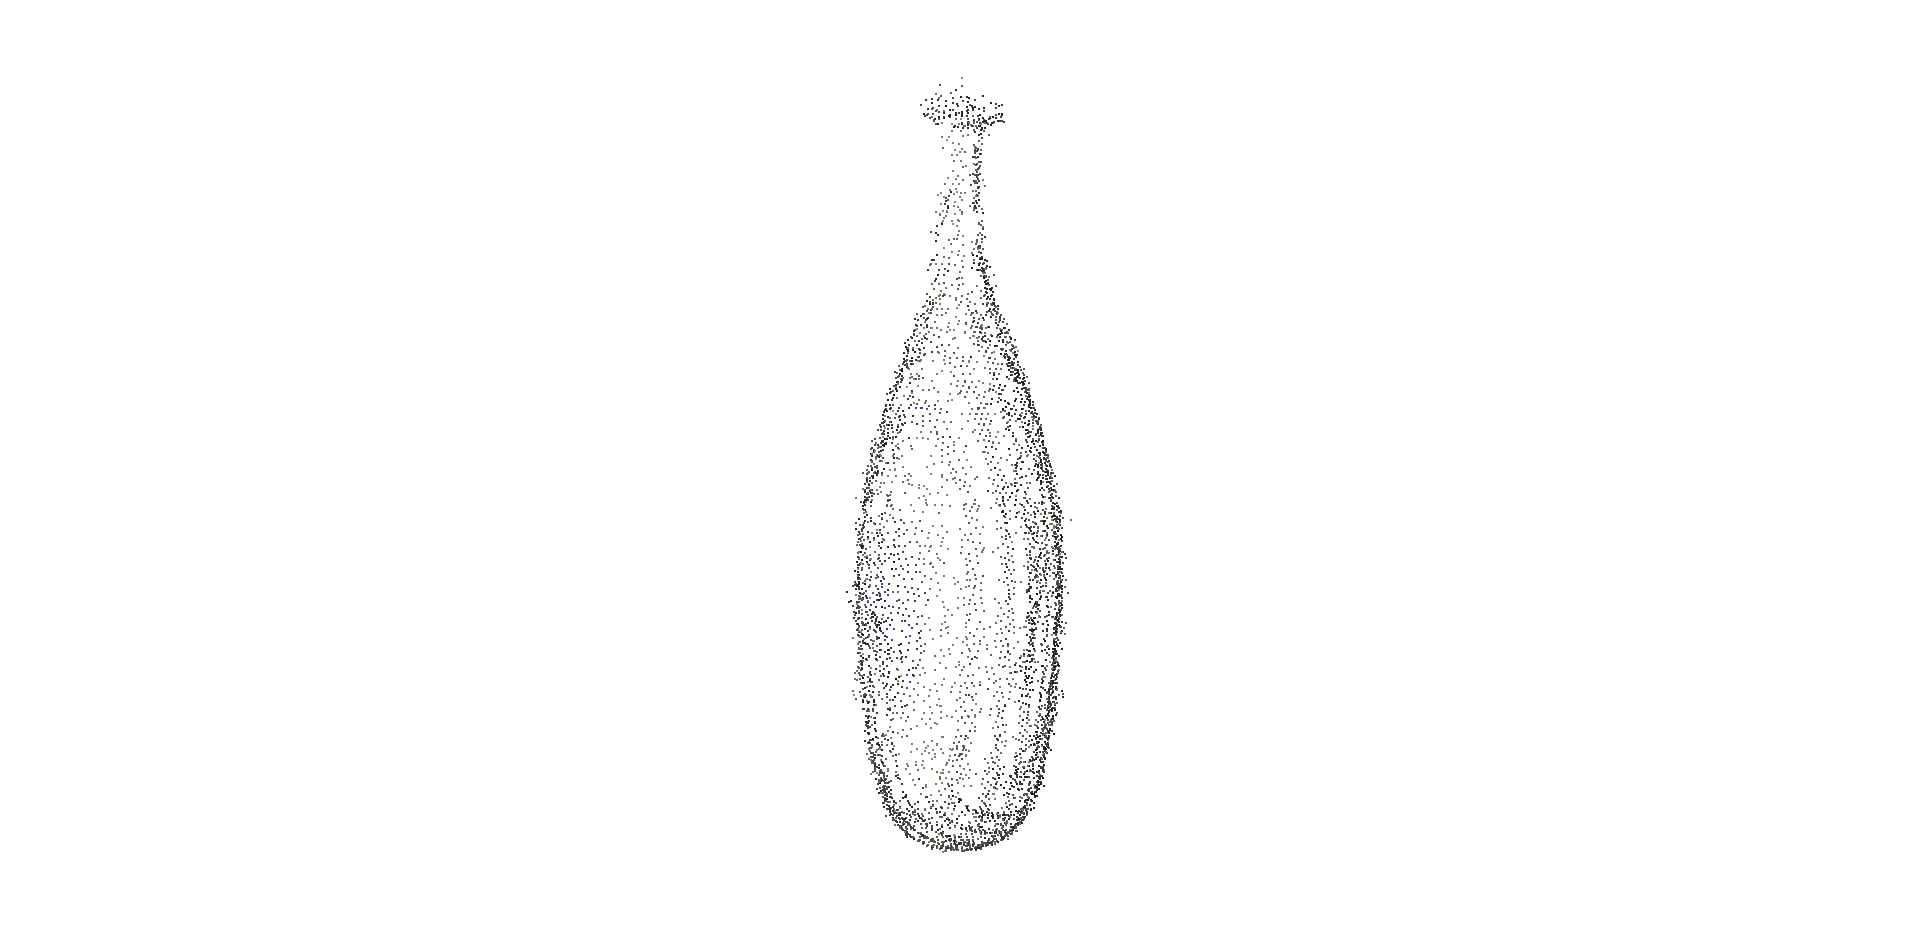
\includegraphics[width=2cm]{interp/synth_data/vase/vase_mvs_02080205.png}&
  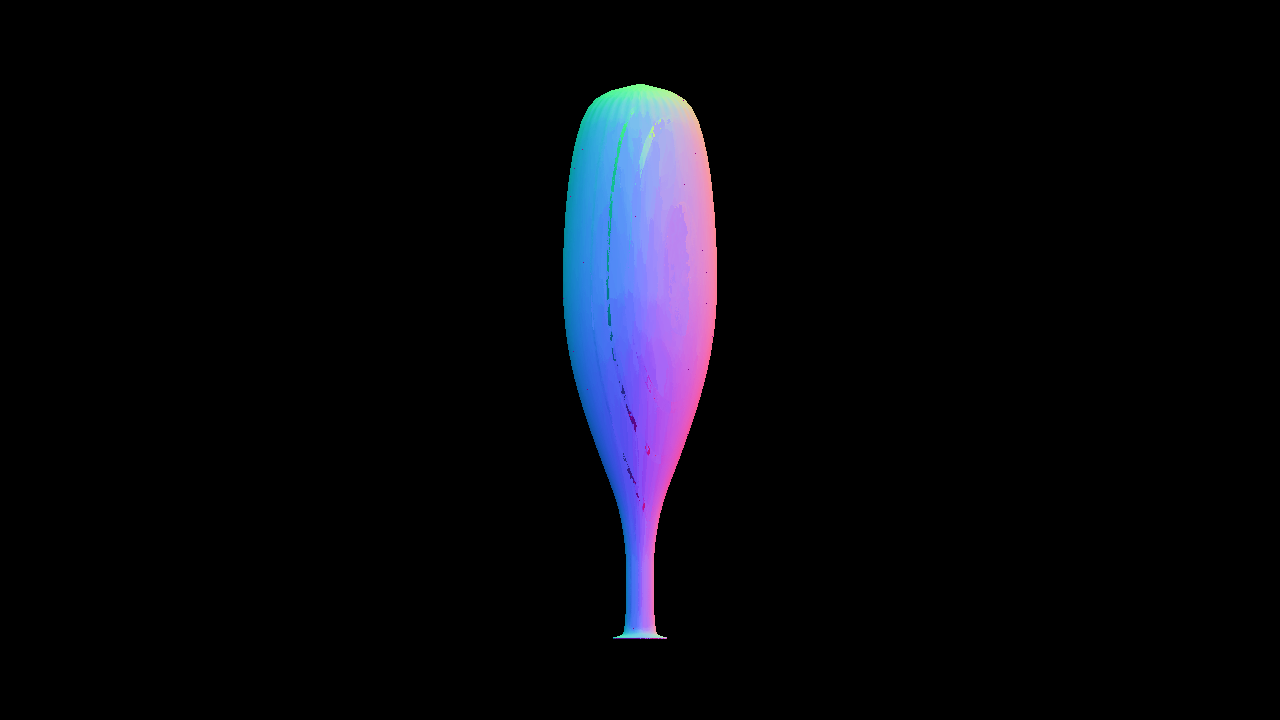
\includegraphics[width=2cm]{interp/synth_data/vase/vase_ps_02080205.png}&
  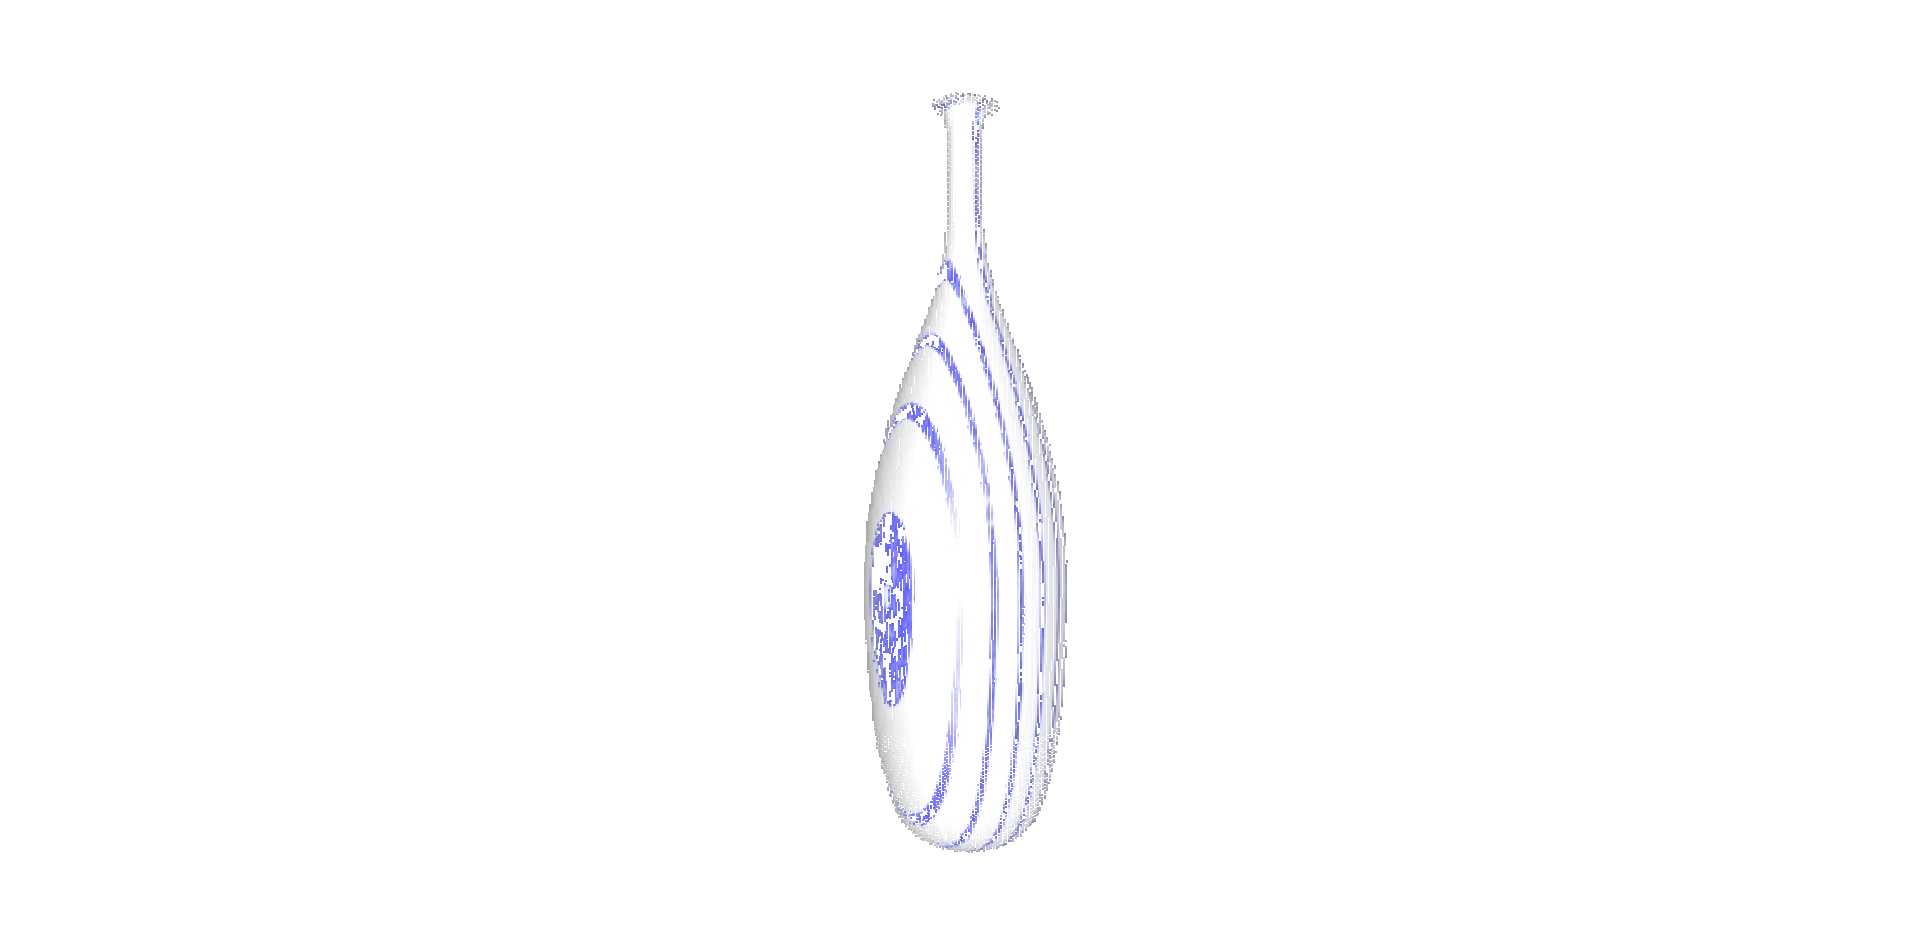
\includegraphics[width=2cm]{interp/synth_data/vase/vase_sl_02080205.png}\\
  ~& MVS & PS & SL\\
\end{tabular}
\caption{Property list: \{tex:0.2, alb:0.8, spec:0.2, rough: 0.5\}. The quantitative and qualitative performance of each technique on three test objects}
\label{fig:test_results_01}
\end{figure}

\textbf{Case 3} MVS performs well, and the completeness of MVS boosted compared to case 1, while the completeness of SL declines from case 1, see Figure~\ref{fig:test_results_02}, which are consistent to the result returned by the abstraction as shown in Table~\ref{tab:prop_list} (c).

\begin{figure}[h!]
\centering
\begin{tabular}{ccccc}
  Quantitative results & ~ & Qualitative results & ~\\
  \includegraphics[width=2cm]{interp/synth_data/cup/cup_08020205}&
  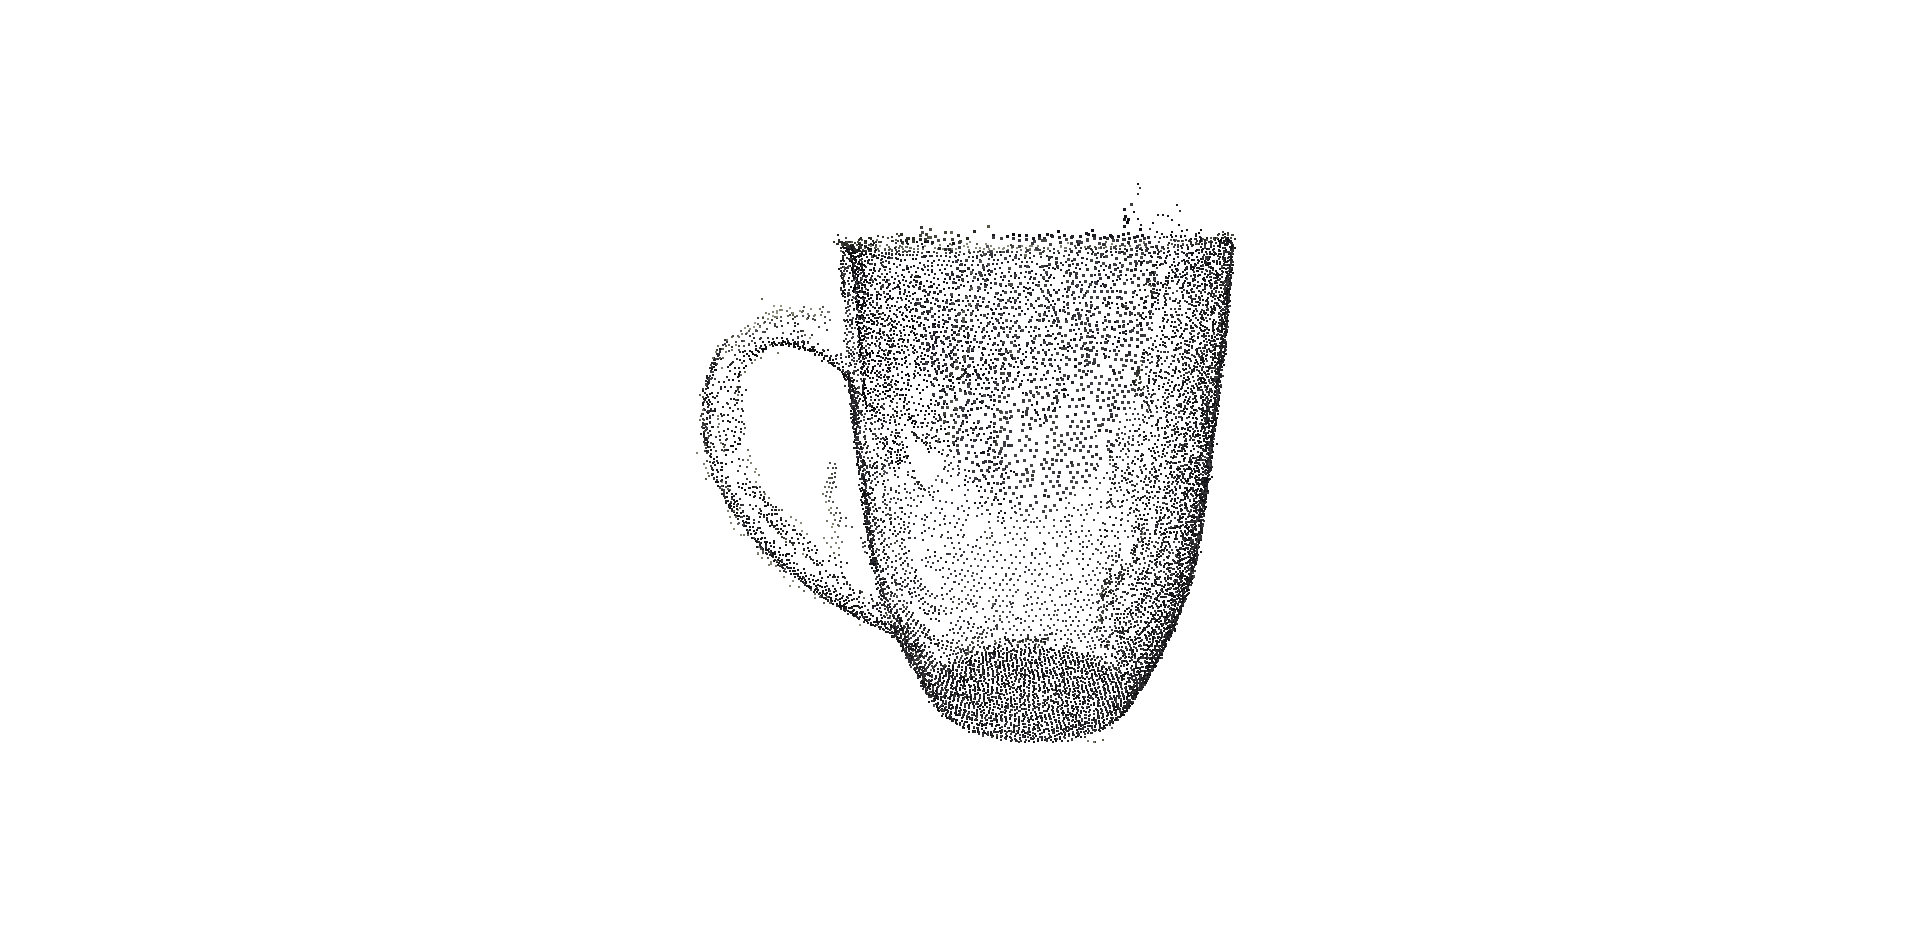
\includegraphics[width=2cm]{interp/synth_data/cup/cup_mvs_08020205.png}&
  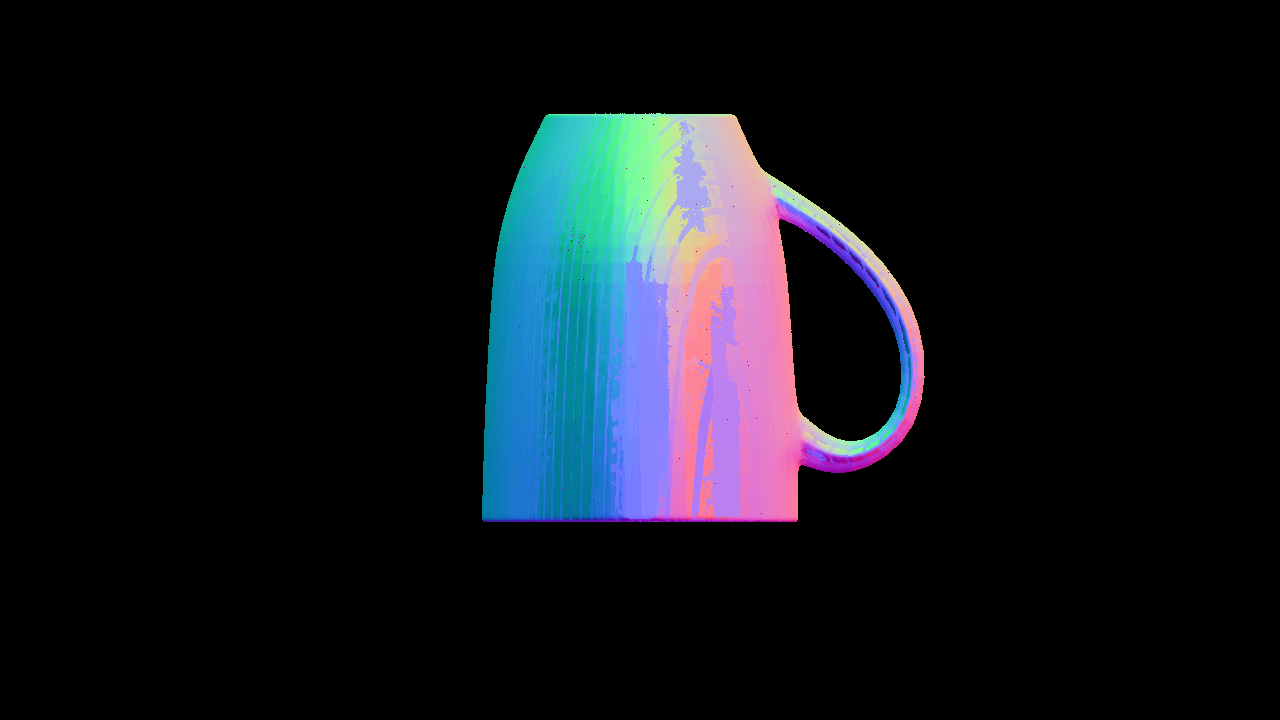
\includegraphics[width=2cm]{interp/synth_data/cup/cup_ps_08020205.png}&
  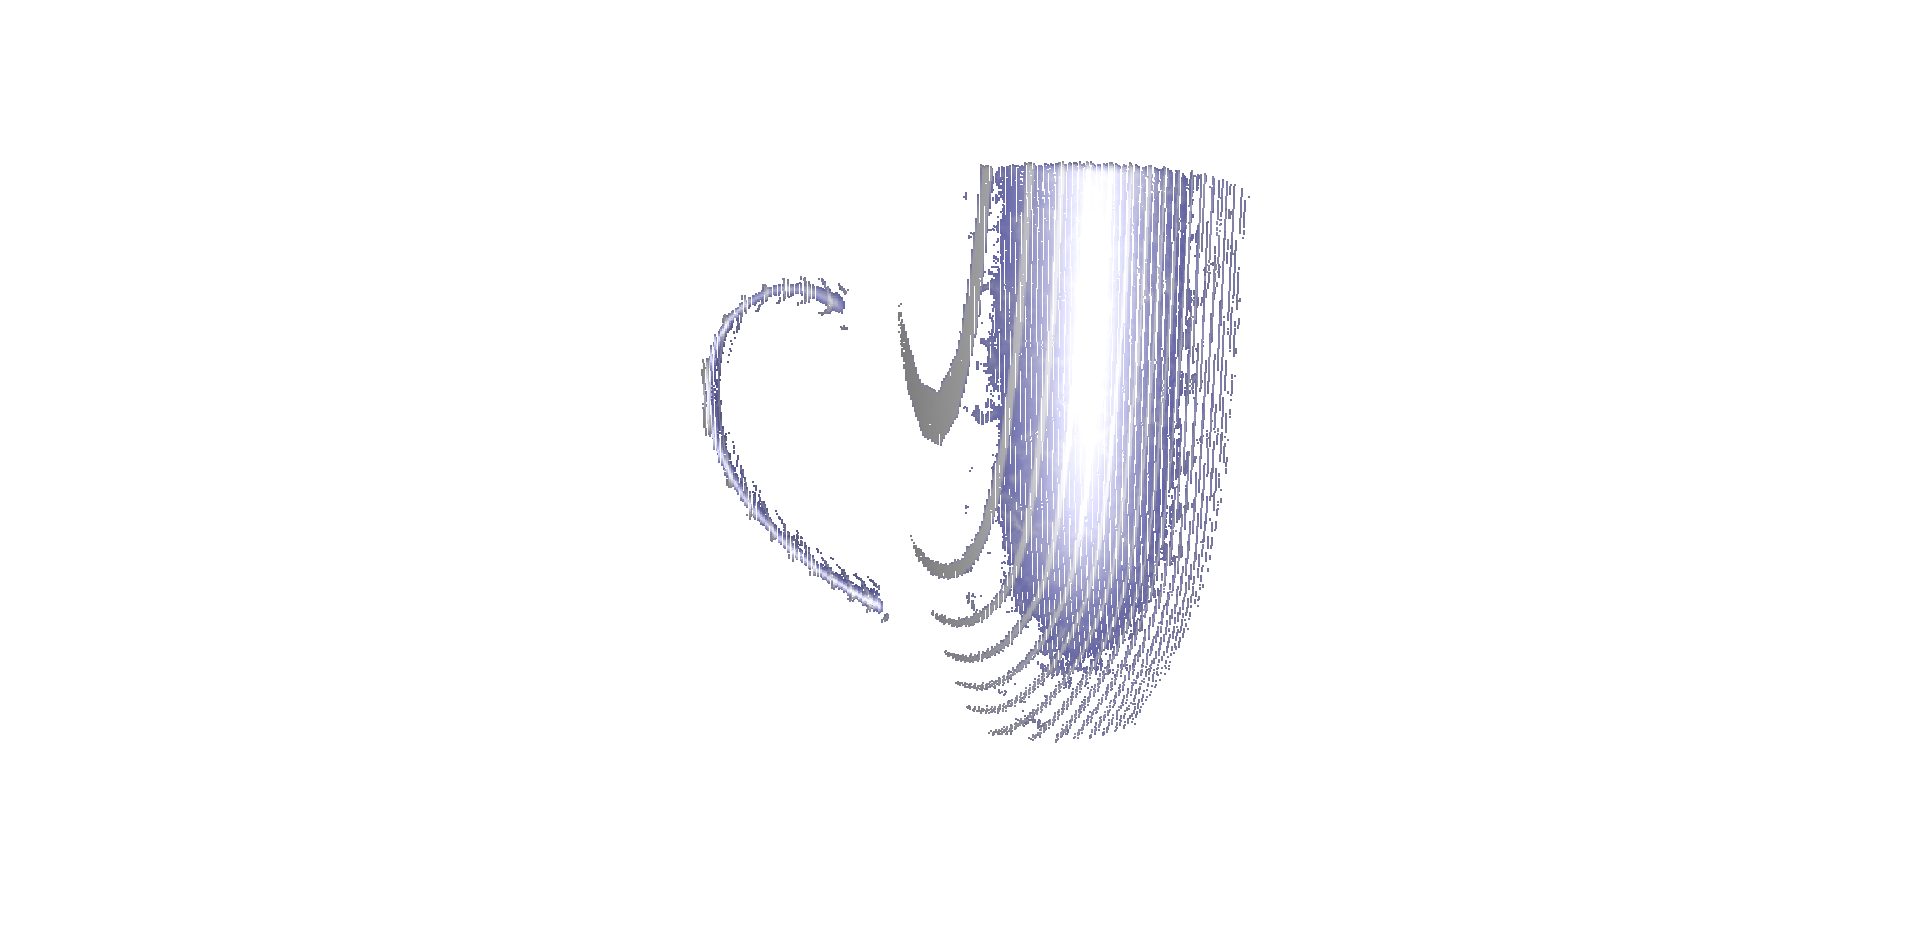
\includegraphics[width=2cm]{interp/synth_data/cup/cup_sl_08020205.png}\\
  \includegraphics[width=2cm]{interp/synth_data/pot/pot_08020205}&
  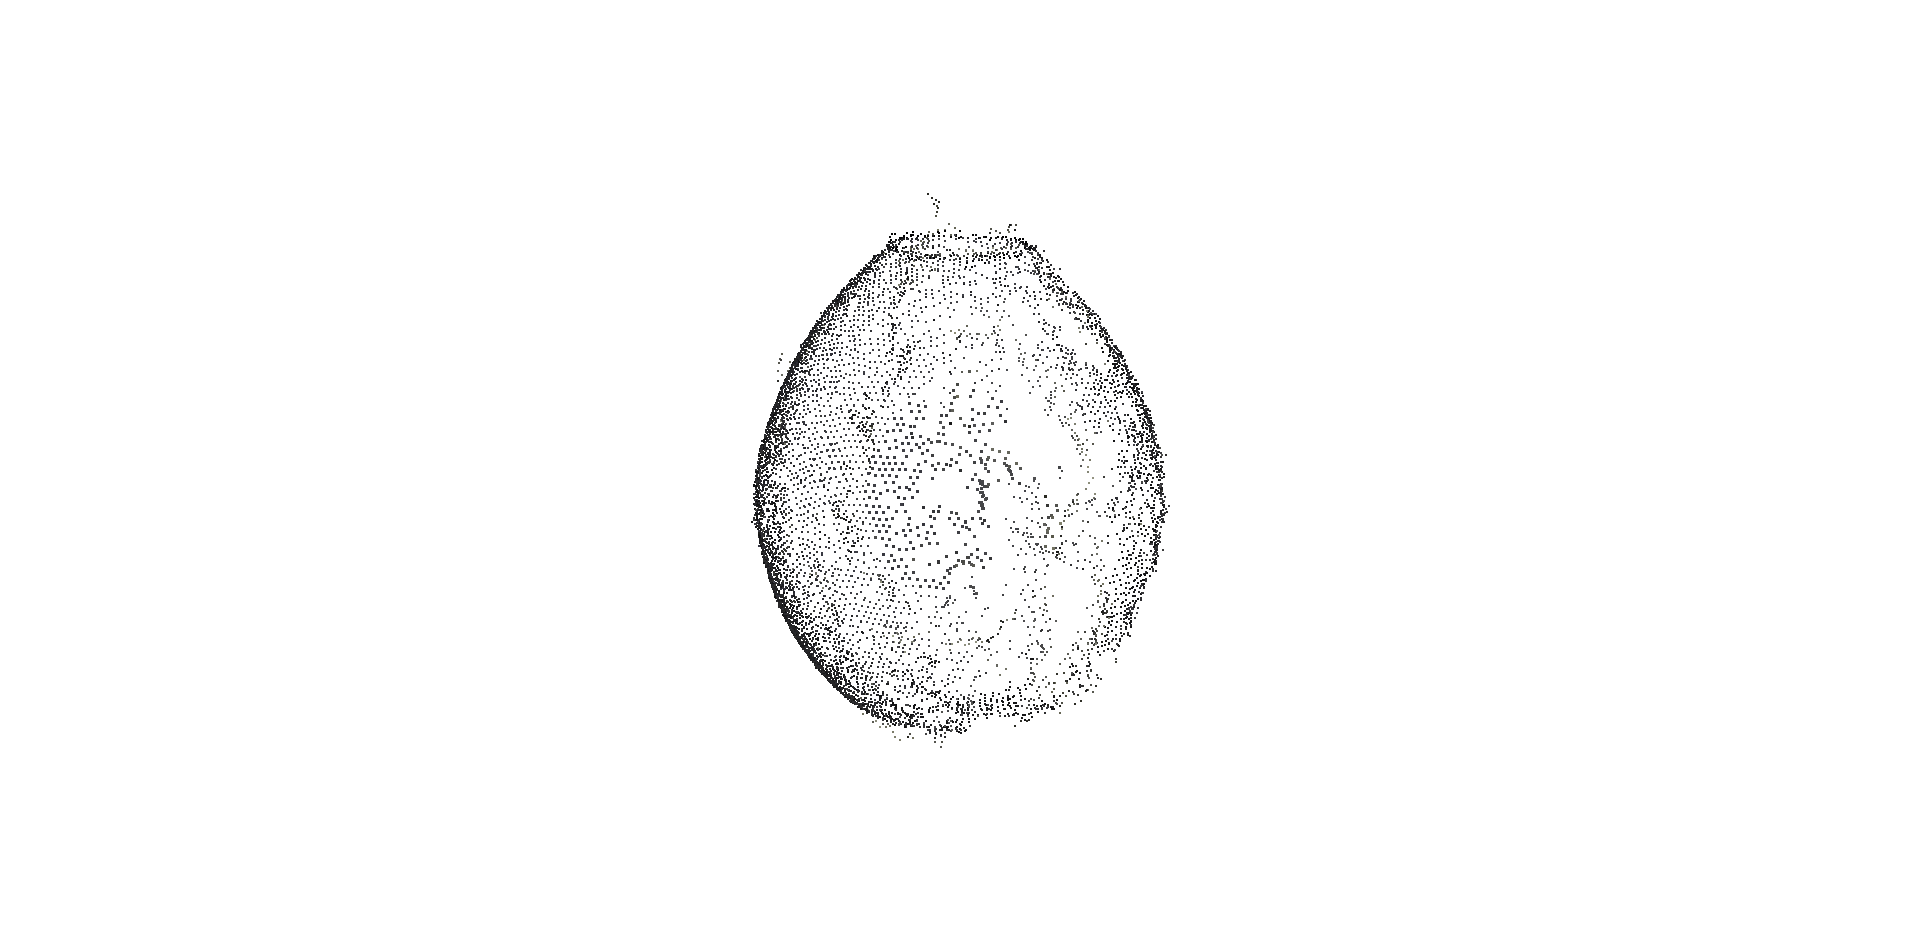
\includegraphics[width=2cm]{interp/synth_data/pot/pot_mvs_08020205.png}&
  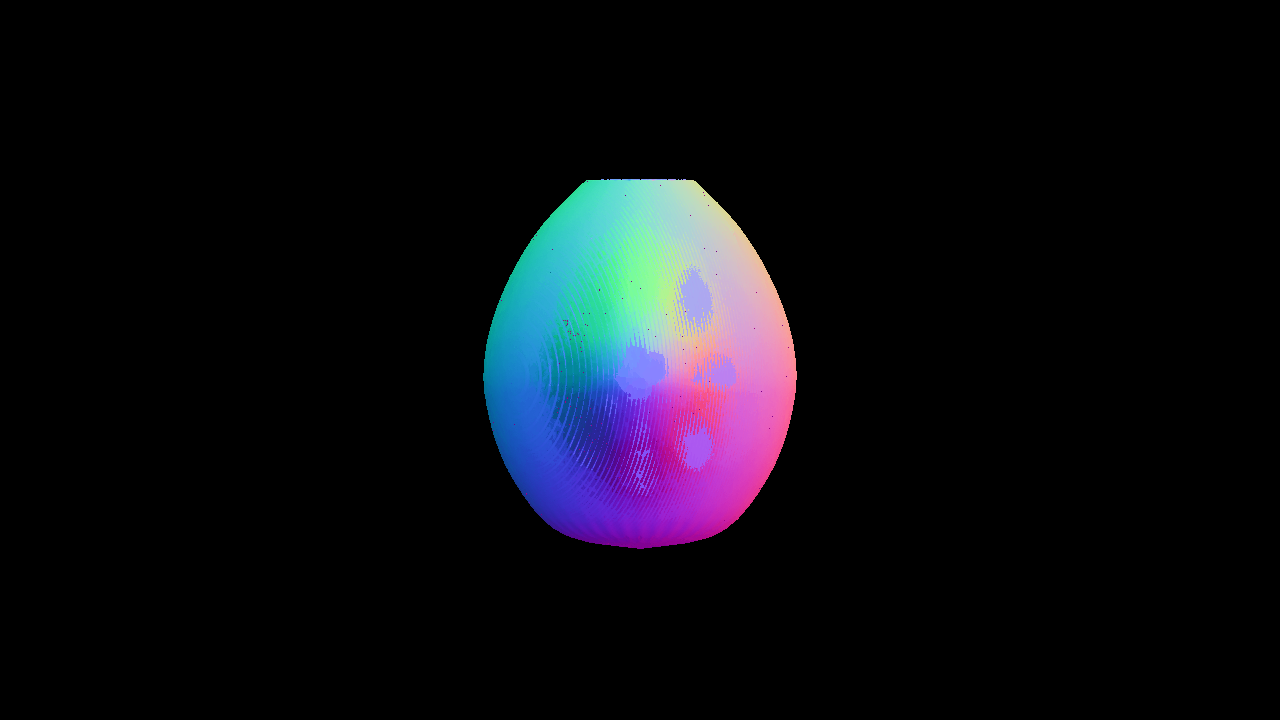
\includegraphics[width=2cm]{interp/synth_data/pot/pot_ps_08020205.png}&
  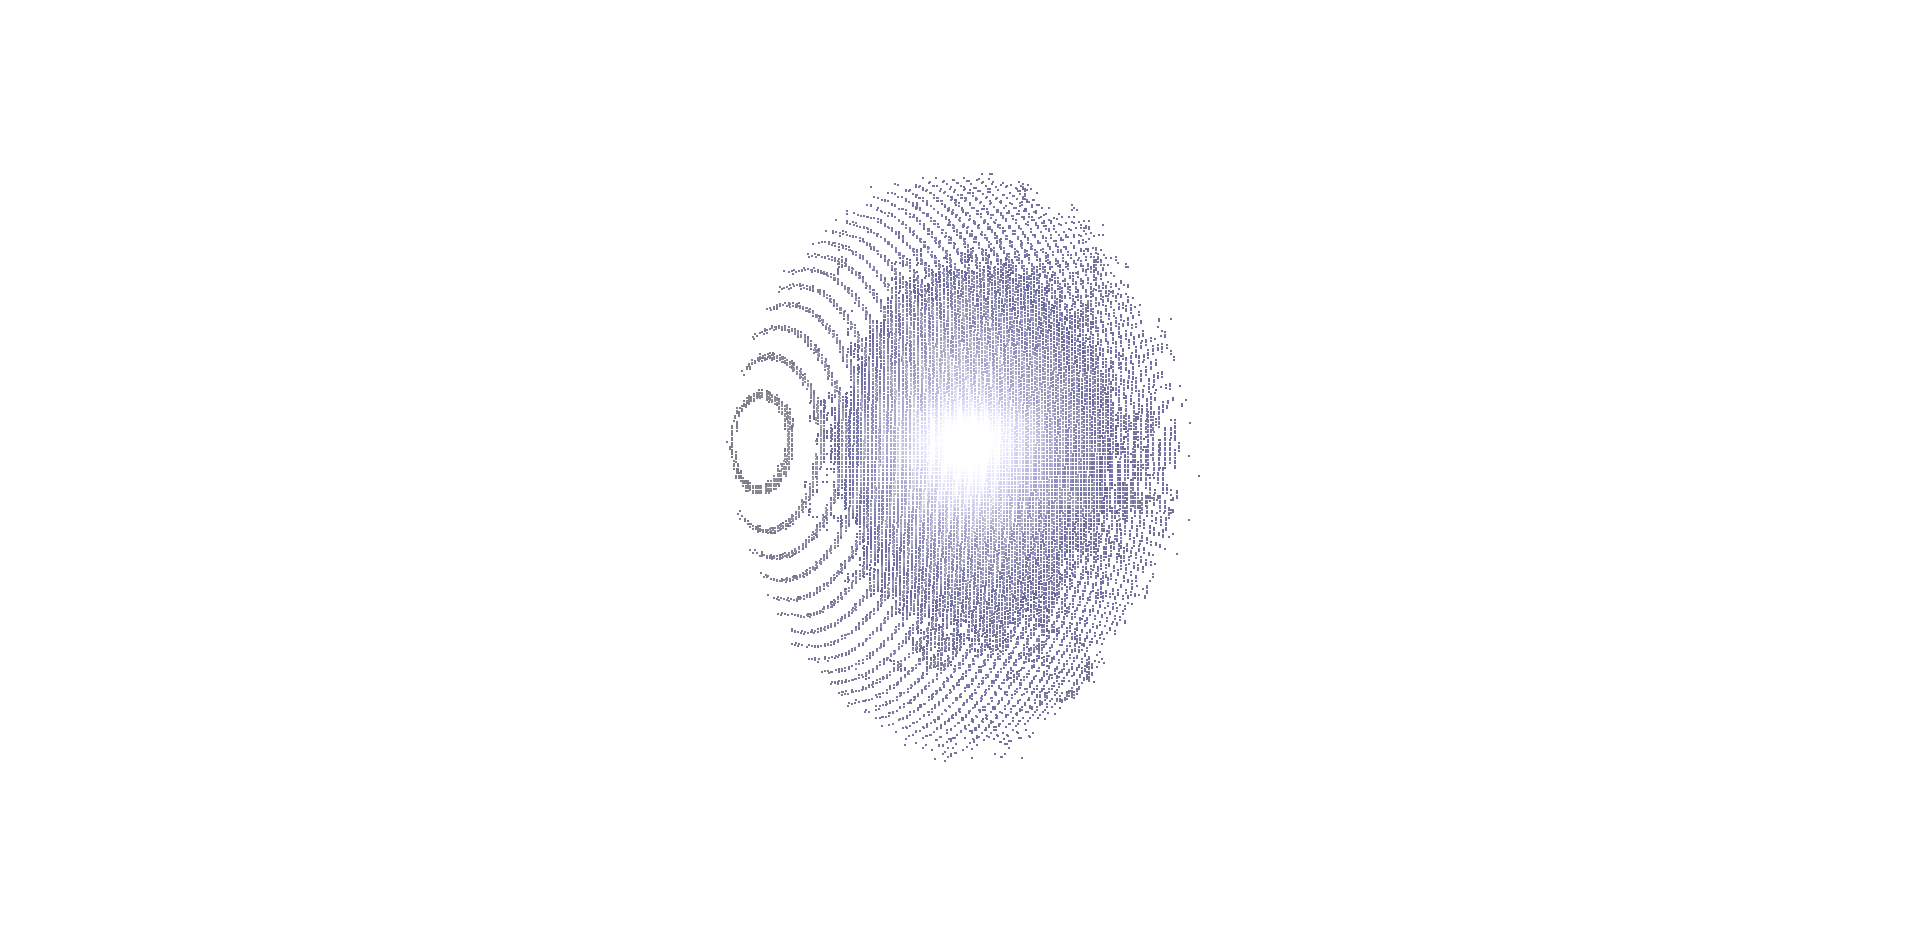
\includegraphics[width=2cm]{interp/synth_data/pot/pot_sl_08020205.png}\\
  \includegraphics[width=2cm]{interp/synth_data/vase/vase_08020205}&
  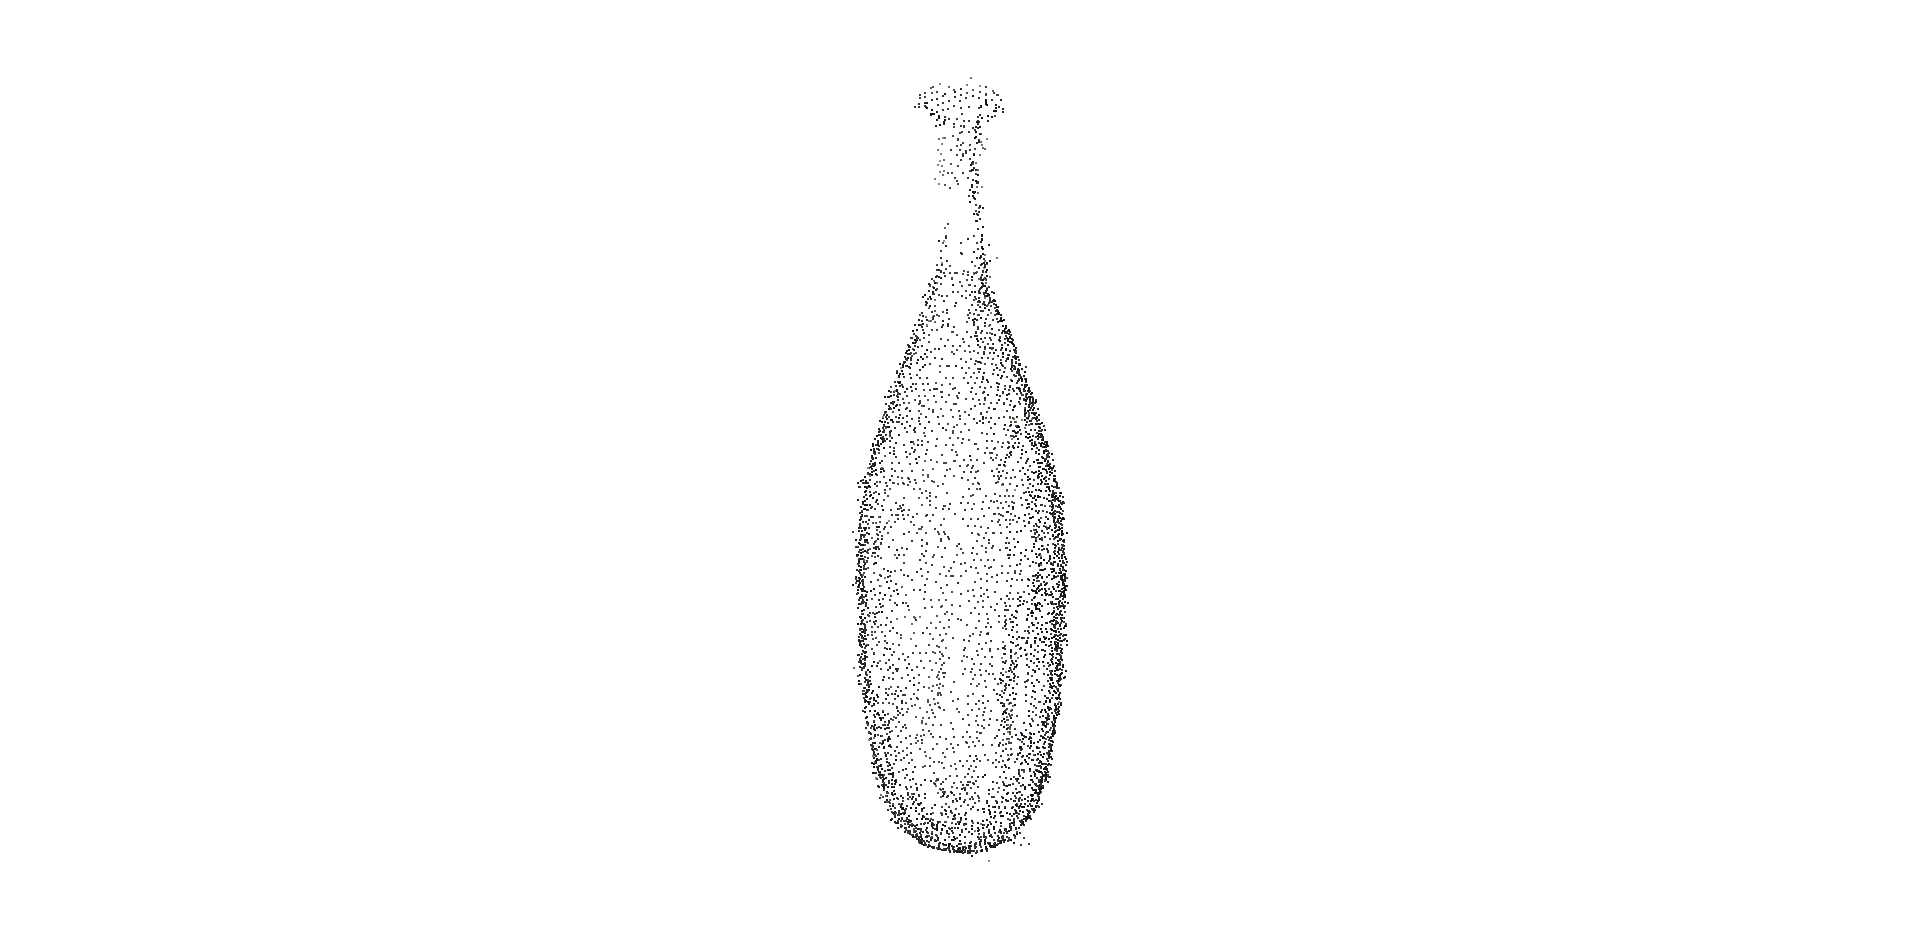
\includegraphics[width=2cm]{interp/synth_data/vase/vase_mvs_08020205.png}&
  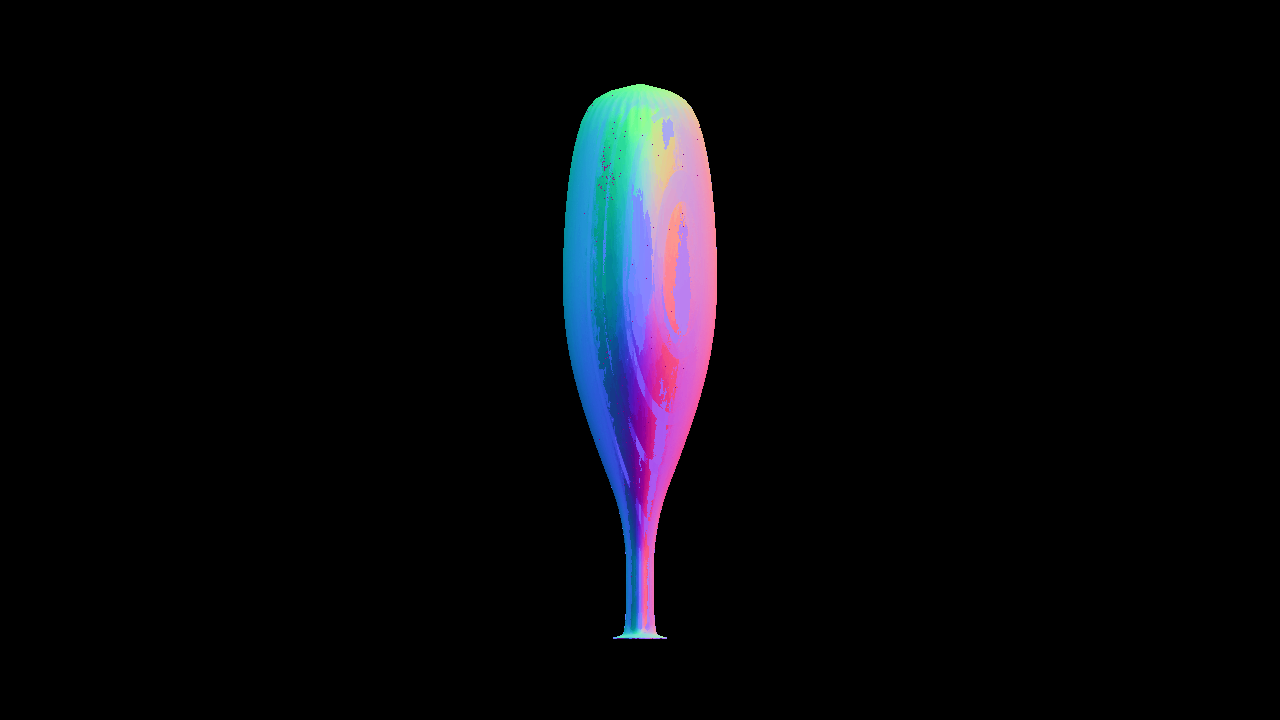
\includegraphics[width=2cm]{interp/synth_data/vase/vase_ps_08020205.png}&
  \includegraphics[width=2cm]{interp/synth_data/vase/vase_sl_08020205.png}\\
  ~& MVS & PS & SL\\
\end{tabular}
\caption{Property list: \{tex:0.8, alb:0.2, spec:0.2, rough: 0.5\}. The quantitative and qualitative performance of each technique on three test objects}
\label{fig:test_results_02}
\end{figure}

\textbf{Case 4} Both MVS and SL perform poorly in this case in terms of completeness. The accuracy of `cup' and `vase' are pretty good, which is not consistent to the abstraction, we argue that it's because their structure is too thin, and both the interior and outside of the cup is textured, which helps improve the accuracy. This shows the need to incorporate more visual and geometric properties to make the abstraction more robust. The PS performs the best among these techniques, which is still consistent to the abstraction as shown in Table~\ref{tab:prop_list} (d). Please refer to Figure~\ref{fig:test_results_03}.

\begin{figure}[h!]
\centering
\begin{tabular}{ccccc}
  Quantitative results & ~ & Qualitative results & ~\\
  \includegraphics[width=2cm]{interp/synth_data/cup/cup_02020802}&
  \includegraphics[width=2cm]{interp/synth_data/cup/cup_mvs_02020802.png}&
  \includegraphics[width=2cm]{interp/synth_data/cup/cup_ps_02020802.png}&
  \includegraphics[width=2cm]{interp/synth_data/cup/cup_sl_02020802.png}\\
  \includegraphics[width=2cm]{interp/synth_data/pot/pot_02020802}&
  \includegraphics[width=2cm]{interp/synth_data/pot/pot_mvs_02020802.png}&
  \includegraphics[width=2cm]{interp/synth_data/pot/pot_ps_02020802.png}&
  \includegraphics[width=2cm]{interp/synth_data/pot/pot_sl_02020802.png}\\
  \includegraphics[width=2cm]{interp/synth_data/vase/vase_02020802}&
  \includegraphics[width=2cm]{interp/synth_data/vase/vase_mvs_02020802.png}&
  \includegraphics[width=2cm]{interp/synth_data/vase/vase_ps_02020802.png}&
  \includegraphics[width=2cm]{interp/synth_data/vase/vase_sl_02020802.png}\\
  ~& MVS & PS & SL\\
\end{tabular}
\caption{Property list: \{tex:0.2, alb:0.2, spec:0.8, rough: 0.2\}. The quantitative and qualitative performance of each technique on three test objects}
\label{fig:test_results_03}
\end{figure}


\section{Real-world Datasets}
We use the dataset `cup' as an example. The property of the `cup' is listed in Table~\ref{tab:prop_list_cup}.

\begin{table}[h]
  \centering
  \begin{tabular}{l*{4}{c}}
  \hline
  \textbf{Property} & Texture coverage & Albedo & Specularity & Roughness\\
  \hline
  cup & 0.2 & 0.8 & 0.8 & 0.2\\
  \hline
  \end{tabular}
  \label{tab:prop_list_cup}
  \caption{Property list for the real-world objects}
\end{table}

From the trained performance of each technique as shown in Figure~\ref{fig:train_cup}
\begin{figure}[h!]
\begin{tabular}{ccc}
\includegraphics[width=0.33\textwidth]{interp/real_data/mvs_train}&
\includegraphics[width=0.33\textwidth]{interp/real_data/ps_train}&
\includegraphics[width=0.33\textwidth]{interp/real_data/sl_train}\\
(MVS) & (PS) & (SL)\\
\end{tabular}
\caption{Performance of MVS, PS, and SL with varied properties}
\label{fig:train_cup}
\end{figure}

From the trained performance, we can clearly see that MVS performs poorly, as it ranks fifth among all 9 combinations, after 020802, 020502, 020805, 020505 (order of property as previously stated), thus we conclude that MVS is not suitable for	`cup'.

From the performance of PS, we can see that it performs well in this case, as the mean and median angle different is below $10^\circ$, and mean and median are not far apart, suggesting that there is no spikes.

From the performance of SL, we can see that it ranks top 3 among all 9 combinations in terms of completeness, thus SL also does a decent job reconstructing `cup'.

Following the same methods, we obtain the best-suited algorithm(s) for all the other objects as shown in Table~\ref{tab:prop_list_real_data}.

\begin{table}[h]
  \centering
  \begin{tabular}{l*{5}{c}}
  \hline
  \textbf{Property} & Texture coverage & Albedo & Specularity & Roughness & Best-suited Algo.\\
  \hline
  box & 0.8 & 0.8 & 0.2 & 0.2 & MVS, SL, PS\\
  cat0 & 0.5 & 0.2 & 0.5 & 0.2 & None\\
  cat1 & 0.2 & 0.2 & 0.8 & 0.2 & None\\
  cup & 0.2 & 0.8 & 0.8 & 0.2 & PS, SL\\
  dino & 0.2 & 0.5 & 0.2 & 0.5 & PS, SL\\
  house & 0.8 & 0.2,0.8 & 0.8 & 0.2 & MVS\\
  pot & 0.5 & 0.2,0.5 & 0.2 & 0.2 & MVS, SL\\
  status & 0.2 & 0.8 & 0.5 & 0.2 & PS, SL\\
  vase & 0.8 & 0.2 & 0.8 & 0.2 & MVS\\
  \hline
  \end{tabular}
  \label{tab:prop_list_real_data}
  \caption{Property list for the real-world objects}
\end{table}

Here we show the reconstruction of the real-world datasets. Since we don't have the ground truth, visual 

\begin{figure}[h!]
\centering
\begin{tabular}{lcccr}
Object & MVS & PS & SL & Best-suited Algo.\\
box &
\raisebox{-.5\height}{\includegraphics[width=0.2\textwidth]{interp/real_data/box/box_mvs_00}}&
\raisebox{-.5\height}{\includegraphics[width=0.2\textwidth]{interp/real_data/box/box_ps_00}}&
\raisebox{-.5\height}{\includegraphics[width=0.2\textwidth]{interp/real_data/box/box_sl_00}}&
MVS, SL, PS\\
cat0 &
\raisebox{-.5\height}{\includegraphics[width=0.2\textwidth]{interp/real_data/cat0/cat0_mvs_00}}&
\raisebox{-.5\height}{\includegraphics[width=0.2\textwidth]{interp/real_data/cat0/cat0_ps_00}}&
\raisebox{-.5\height}{\includegraphics[width=0.2\textwidth]{interp/real_data/cat0/cat0_sl_00}}&
None\\
cat1 &
\raisebox{-.5\height}{\includegraphics[width=0.2\textwidth]{interp/real_data/cat1/cat1_mvs_00}}&
\raisebox{-.5\height}{\includegraphics[width=0.2\textwidth]{interp/real_data/cat1/cat1_ps_00}}&
\raisebox{-.5\height}{\includegraphics[width=0.2\textwidth]{interp/real_data/cat1/cat1_sl_00}}&
None\\
dino &
\raisebox{-.5\height}{\includegraphics[width=0.2\textwidth]{interp/real_data/dino/dino_mvs_00}}&
\raisebox{-.5\height}{\includegraphics[width=0.2\textwidth]{interp/real_data/dino/dino_ps_00}}&
\raisebox{-.5\height}{\includegraphics[width=0.2\textwidth]{interp/real_data/dino/dino_sl_00}}&
PS, SL\\
cup &
\raisebox{-.5\height}{\includegraphics[width=0.2\textwidth]{interp/real_data/cup/cup_mvs_00}}&
\raisebox{-.5\height}{\includegraphics[width=0.2\textwidth]{interp/real_data/cup/cup_ps_00}}&
\raisebox{-.5\height}{\includegraphics[width=0.2\textwidth]{interp/real_data/cup/cup_sl_00}}&
PS, SL\\
house &
\raisebox{-.5\height}{\includegraphics[width=0.2\textwidth]{interp/real_data/house/house_mvs_00}}&
\raisebox{-.5\height}{\includegraphics[width=0.2\textwidth]{interp/real_data/house/house_ps_00}}&
\raisebox{-.5\height}{\includegraphics[width=0.2\textwidth]{interp/real_data/house/house_sl_00}}&
MVS\\
pot &
\raisebox{-.5\height}{\includegraphics[width=0.2\textwidth]{interp/real_data/pot/pot_mvs_01}}&
\raisebox{-.5\height}{\includegraphics[width=0.2\textwidth]{interp/real_data/pot/pot_ps_00}}&
\raisebox{-.5\height}{\includegraphics[width=0.2\textwidth]{interp/real_data/pot/pot_sl_00}}&
MVS, SL\\
\end{tabular}
\caption{Reconstruction results of MVS, PS, SL}
\label{fig:test_real_world_obj}
\end{figure}

\begin{figure}[h!]
\centering
\begin{tabular}{lcccr}
Object & MVS & PS & SL & Best-suited Algo.\\
statue &
\raisebox{-.5\height}{\includegraphics[width=0.2\textwidth]{interp/real_data/statue/statue_mvs_00}}&
\raisebox{-.5\height}{\includegraphics[width=0.2\textwidth]{interp/real_data/statue/statue_ps_00}}&
\raisebox{-.5\height}{\includegraphics[width=0.2\textwidth]{interp/real_data/statue/statue_sl_00}}&
PS, SL\\
vase &
\raisebox{-.5\height}{\includegraphics[width=0.2\textwidth]{interp/real_data/vase/vase_mvs_01}}&
\raisebox{-.5\height}{\includegraphics[width=0.2\textwidth]{interp/real_data/vase/vase_ps_00}}&
\raisebox{-.5\height}{\includegraphics[width=0.2\textwidth]{interp/real_data/vase/vase_sl_00}}&
MVS\\
\end{tabular}
\caption{Reconstruction results of MVS, PS, SL (cont'd)}
\label{fig:test_real_world_obj}
\end{figure}

\section{Observations}
\begin{itemize}
\item roughness on ps
\item low albedo, high specularity on SL
\item low albedo, high specularity, low roughness, high spikes
\end{itemize}

\section{Summary}

